% Paquets généraux
\documentclass[a4paper,12pt,titlepage,twoside]{article}
\usepackage[T1]{fontenc}
\usepackage[utf8]{inputenc}
\usepackage[french]{babel}
\usepackage{subcaption}
\addto\captionsfrench{%
  \renewcommand{\tablename}{Tableau}%
}
\usepackage[gen]{eurosym}
%\usepackage[dvips]{graphicx}
\usepackage{minted}
\usepackage{fancyhdr}
\usepackage{pdfpages} 
\usepackage{multido}
\usepackage{hyperref}
\usepackage{textcomp}
\usepackage{schemabloc}
%\usepackage[bitstream-charter]{mathdesign}
\usepackage{array}
\newcolumntype{P}[1]{>{\centering\arraybackslash}p{#1}}
\usepackage[shortlabels]{enumitem}
\usepackage[framemethod=TikZ]{mdframed}

\newcommand{\id}{71}
\newcommand{\nom}{Théorie des mécanismes}
\newcommand{\sequence}{04}
\newcommand{\nomsequence}{Liaisons entre les solides}
\newcommand{\num}{02}
\newcommand{\type}{KH}
\newcommand{\descrip}{Liaisons équivalentes, hyperstatisme, liaisons en série et en parallèle, théorie des graphes}
\newcommand{\competences}{B2-12: Proposer une modélisation des liaisons avec leurs caractéristiques géométriques. \\ &  B2-13: Proposer un modèle cinématique paramétré à partir d'un système réel, d'une maquette numérique ou d'u \\ &  B2-17: Simplifier un modèle de mécanisme. \\ &  B2-18: Modifier un modèle pour le rendre isostatique. \\ &  C1-04: Proposer une démarche permettant d'obtenir une loi entrée-sortie géométrique.  \\ &  C2-05: Caractériser le mouvement d'un repère par rapport à un autre repère. \\ &  C2-06: Déterminer les relations entre les grandeurs géométriques ou cinématiques. }
\newcommand{\nbcomp}{7}
\newcommand{\systemes}{}
\newcommand{\systemesnum}{}
\newcommand{\systemessansaccent}{}
\newcommand{\ilot}{2}
\newcommand{\ilotstr}{02}
\newcommand{\dossierilot}{\detokenize{Ilot_02 }}

%\usepackage{style}
\usepackage{bodegraph}
\usepackage{rpcinematik}
\usepackage[locale = FR]{siunitx}
\usepackage{caption}
\newcommand{\institute}{Lycée Dorian}

\usepackage{listings}
\usepackage{fancyvrb}
\usepackage{color}
\usepackage{xcolor}
\usepackage{colortbl}
\usepackage{helvet}
\usepackage[frenchmath]{newtxsf} % for sans serif symbols
\renewcommand{\familydefault}{\sfdefault}
%\usepackage{amsfonts}
%\usepackage{amsmath}
%\usepackage{lmodern}
\usepackage{mathastext}
%\usepackage{xspace}
\usepackage{varioref}
\usepackage{tabularx}
%\usepackage{floatflt}
\usepackage{graphics}
\usepackage{wrapfig}
\usepackage{textcomp}
\usepackage{tikz,tkz-tab}
\usepackage[european resistor, european voltage, european current]{circuitikz}
\usepackage{wrapfig}
\usepackage{gensymb}
\usepackage[percent]{overpic}
\usetikzlibrary{babel}
\usepackage{ifthen}
\usepackage{cancel}
\usepackage{etoolbox}
\usepackage{multirow}
%\usepackage{boxedminipage}
\definecolor{gris25}{gray}{0.75}
\definecolor{bleu}{RGB}{18,33,98}
\definecolor{bleuf}{RGB}{42,94,171}
\definecolor{bleuc}{RGB}{231,239,247}
\definecolor{bleum}{RGB}{160,195,226}
\definecolor{rougef}{RGB}{185,18,27}
\definecolor{rougec}{RGB}{255,188,204}%255,230,231
\definecolor{vertf}{RGB}{103,126,82}
\definecolor{vertc}{RGB}{220,255,191}
\definecolor{forestgreen}{rgb}{0.13,0.54,0.13}
\definecolor{blcr}{rgb}{0.59,0.69,0.84}
\definecolor{blfr}{rgb}{0.32,0.51,0.75}
\definecolor{orfr}{rgb}{0.90,0.42,0.15}
\definecolor{orcr}{rgb}{0.90,0.65,0.50}
\definecolor{orangef}{rgb}{0.659,0.269,0.072}
\definecolor{orange}{rgb}{0.58,0.35,0.063}
\definecolor{orangec}{rgb}{0.43,0.32,0.25}
\definecolor{rcorrect}{rgb}{0.6,0,0}
\definecolor{sequence}{rgb}{0.75,0.75,0.75}
\definecolor{competences}{rgb}{0.61,0.73,0.35}
\definecolor{rose}{HTML}{ff00ff}
\definecolor{grisf}{HTML}{222222}
\definecolor{grisc}{HTML}{636363}
\definecolor{normal}{HTML}{4087c4}
\definecolor{info}{HTML}{5bc0de}
\definecolor{success}{RGB}{92,184,92}
\definecolor{warning}{RGB}{240,173,78}
\definecolor{danger}{RGB}{217,83,79}
\hypersetup{                    % parametrage des hyperliens
    colorlinks=true,                % colorise les liens
    breaklinks=true,                % permet les retours à la ligne pour les liens trop longs
    urlcolor= blfr,                 % couleur des hyperliens
    linkcolor= orange,                % couleur des liens internes aux documents (index, figures, tableaux, equations,...)
    citecolor= forestgreen                % couleur des liens vers les references bibliographiques
    }

\newcolumntype{M}[1]{>{\centering\arraybackslash}m{#1}}
\definecolor{codegreen}{rgb}{0,0.6,0}
\definecolor{codegray}{rgb}{0.5,0.5,0.5}
\definecolor{codepurple}{rgb}{0.58,0,0.82}
\definecolor{backcolour}{rgb}{0.95,0.95,0.92}

\lstdefinestyle{mystyle}{
    backgroundcolor=\color{backcolour},   
    commentstyle=\color{codegreen},
    keywordstyle=\color{magenta},
    numberstyle=\tiny\color{codegray},
    stringstyle=\color{codepurple},
    basicstyle=\ttfamily\footnotesize,
    breakatwhitespace=false,         
    breaklines=true,                 
    captionpos=b,                    
    keepspaces=true,                 
    numbers=left,                    
    numbersep=5pt,                  
    showspaces=false,                
    showstringspaces=false,
    showtabs=false,                  
    tabsize=2
}

\lstset{style=mystyle}

% Mise en page
\pagestyle{fancy}

\setlength{\hoffset}{-18pt}
\setlength{\oddsidemargin}{0pt} 	% Marge gauche sur pages impaire2s
\setlength{\evensidemargin}{0pt} 	% Marge gauche sur pages paires
\setlength{\marginparwidth}{00pt} 	% Largeur de note dans la marge
\setlength{\headwidth}{481pt} 	 	% Largeur de la zone de tête (17cm)
\setlength{\textwidth}{481pt} 	 	% Largeu\textbf{r de la zone de texte (17cm)
\setlength{\voffset}{-18pt} 		% Bon pour DOS
\setlength{\marginparsep}{7pt}	 	% Séparation de la marge
\setlength{\topmargin}{-30pt} 		% Pas de marge en haut
\setlength{\headheight}{55pt} 		% Haut de page
\setlength{\headsep}{20pt} 		% Entre le haut de page et le texte
\setlength{\footskip}{30pt} 		% Bas de\textbf{ page + séparation
\setlength{\textheight}{700pt} 		% Hauteur de l'icone zone de texte (25cm)
\setlength\fboxrule{1 pt}
\renewcommand{\baselinestretch}{1}
\setcounter{tocdepth}{1}
\newcommand{\cadre}[2]
{\fbox{
  \begin{minipage}{#1\linewidth}
   \begin{center}
    #2\\
   \end{center}
  \end{minipage}
 }
}

\newcommand{\repon}[1]
{
~\ \\
\begin{tabular}{|m{\linewidth}|}
 \hline
\multido{}{#1}{\\ \hline}
\end{tabular}
}


\newcommand{\objectif}[1]{
\mdfsetup{%
frametitle={%
\tikz[baseline=(current bounding box.east),outer sep=0pt]
\node[anchor=east,rectangle,fill=bleum]
{\strut Objectif~};}}
\mdfsetup{innertopmargin=10pt,linecolor=bleum,%
linewidth=2pt,topline=true,%
frametitleaboveskip=\dimexpr-\ht\strutbox\relax
}
\begin{mdframed}[]\relax%
#1
\end{mdframed}}


\newcounter{num_quest} \setcounter{num_quest}{0}
\newcounter{num_rep} \setcounter{num_rep}{0}
\newcounter{num_cor} \setcounter{num_cor}{0}

\newcommand{\feuilleDR}[1]{
	\begin{tikzpicture}
		\draw[gray!30](0,0)grid[step=0.5cm](\linewidth,#1);
	\end{tikzpicture}
}

%\newcommand{\question}[1]{\refstepcounter{num_quest}\par
%~\ \\ \parbox[t][][t]{0.15\linewidth}{\textbf{Question \arabic{num_quest}}}\parbox[t][][t]{0.85\linewidth}{#1\label{q\the\value{num_quest}}}\par
%}

\newcommand{\question}[1]{\refstepcounter{num_quest}\par
~\ \\ \textbf{Question \arabic{num_quest} : }#1\label{q\the\value{num_quest}}\par
}

\newcommand{\posetafigure}[3]{
\begin{figure}[ht!]
 \begin{center}
  \includegraphics[width=#2\linewidth]{img/#1}
 \end{center}
 \caption{\label{#1} #3}
\end{figure}}

\newcommand{\goforum}{
\begin{figure}

\end{figure}
\begin{center}
 
\includegraphics[width=0.7\linewidth]{../../../img/go_forum}
\end{center}
\label{go_forum}
\caption{J'pète les plombs}
\end{figure}}

\newcommand{\reponse}[4][1]
{\noindent
\parbox{\textwidth}{
\rule{\linewidth}{.5pt}\\
\textbf{Question\ifthenelse{#1>1}{s}{} \multido{}{#1}{%
\refstepcounter{num_rep}\ref{q\the\value{num_rep}} }:} ~\ \\
\ifdef{\public}{#3 \ifthenelse{#2>0}{~\ \\ 	\feuilleDR{#2}}}{#4}
}}

\newcommand{\cor}
{\refstepcounter{num_cor}
\noindent
\rule{\linewidth}{.5pt}
\textbf{Question \arabic{num_cor}:} \\
}

\newcommand{\finsujet}
{
    \begin{center}
    \Large{FIN}
    \end{center}

    \cleardoublepage

    \ifdef{\public}{\pagestyle{docreponse}}{\pagestyle{correction}}

    \ifdef{\public}{
        \begin{tikzpicture} 
            \draw (0,0) rectangle (2,2);
            \draw (0,0) -- (2,2);
            \draw (1.5,0.5) node {\large 20};
            \draw (2.5,0) rectangle (16,2);
            \draw (4.5,1.7) node {\large Commentaires:};
        \end{tikzpicture}
    }
    ~\ \\
}


%\newcommand{\repcarre}[2]
%{
%~\ \\
%\begin{tikzpicture}
%\draw [fill=white] (0,0) rectangle +(\linewidth,#1);
%\node[align=left] at (1.1,#2-0.3) {\textbf{Question #1:}};
%\end{tikzpicture}
%}

\newcommand{\titre}[1]
{\begin{center}
\cadre{0.8}{\huge #1} 
\end{center}
}


%Définition des torseurs :
\newcommand{\torseur}[2]{\left\{\mathcal{#1}_{#2} \right\}}
\newcommand{\torseurh}[3]{\left\{\genfrac{}{}{0pt}{0}{#1}{#2}\right\}_{#3}}
\newcommand{\torseurv}[8]{\left\{
\begin{matrix}
#1 & #4 \\ #2 & #5 \\ #3 &#6
\end{matrix}
\right\}_{{#7},{#8}}}

%Définition des torseurs :
%\newcommand{\torseur}[2]{\left \{\mbox{\relsize{2}{$\mathcal {#1}$}\relsize{-2}}\phantom{}_{\mbox{\scriptsize $#2$}} \right \}}
%\newcommand{\torseurh}[3]{\left\{\genfrac{}{}{0pt}{0}{#1}{#2}\right\}_{#3}}
%\newcommand{\torseurv}[8]{
%\left\{\begin{array}{@{}c|c@{}} #1 & #4 \\ #2 & #5 \\ #3 & #6 \end{array} \right\}_{#7,#8}
%}
\newcommand{\derivee}[2]{\left.\dfrac{\d #1}{\d t}\right|_{#2}}
\newcommand{\tripleint}{\int\!\!\!\!\!\int\!\!\!\!\!\int}

% Notation cinématique et statique
\newcommand{\cinematique}[2]{\mbox{#1}/\mbox{#2}}
\newcommand{\statique}[2]{\mbox{#1}\rightarrow\mbox{#2}}
\newcommand{\moment}[3]{\vv {#1}_{\scriptsize{#3}}(#2)}
\newcommand{\resultante}[2]{\vv {#1}_{\scriptsize{#2}}}


%Commande de base
\newcommand{\jo}{\left(j\omega\right)} % j \omega dans l'analyse fréquentielle
\newcommand{\tl}{\xrightarrow{\mathcal{L}}} % transformée de laplace sur fleche
\newcommand{\tli}{\xrightarrow{\mathcal{L}^{-1}}} % transformée inverse de laplace sur fleche
\renewcommand{\d}[1][]{\mathrm{d#1}}
\newcommand{\dd}[1][]{\mathrm{d#1}}
\newcommand{\vect}[2]{{#1}\wedge{#2}}
\newcommand{\base}[3]{(\vec #1,\vec #2,\vec #3)}
\newcommand{\vectbase}[4]{{\vphantom{\left| \begin{matrix}
#1\\#2\\#3 \end{matrix} \right|}}_{#4}{\left| \begin{matrix}
#1\\#2\\#3 \end{matrix} \right.}}
%Pour avoir les paragraphes sous la forme I, II, III
\renewcommand{\thesection}{\Roman{section}}
\setcounter{secnumdepth}{3}
\renewcommand{\Frlabelitemii}{$\bullet$}

% En tête et pied de page
\lhead{\nom}
\rhead{
\includegraphics[width=2cm]{../../../img/logo}}
\lfoot{\auteurun,\ \auteurdeux}
\cfoot{Page \thepage}

\fancypagestyle{docreponse}{%
  \fancyhf{}
  \fancyhead[LO]{NOM Prénom: .............................}
  \rhead{
\includegraphics[width=2cm]{../../../img/logo}\hspace{2pt}}
  \ifdef{\auteurdeux}{\lfoot{\auteurun,\ \auteurdeux}}{\lfoot{\auteurun}}
  \rfoot{\nom}
  \lfoot{Document réponse}
  \cfoot{Page \thepage}
   }

\fancypagestyle{correction}{%
  \fancyhf{}
  \lhead{\colorbox{danger}{\begin{minipage}{0.65\paperwidth} \textcolor{white}{\textbf{Correction}} \end{minipage}} }
  \rhead{
\includegraphics[width=2cm]{../../../img/logo}}
  \lfoot{Renaud Costadoat, Françoise Puig}
  \rfoot{\colorbox{danger}{\begin{minipage}{0.4\paperwidth} \begin{flushright}\textcolor{white}{\textbf{Correction}}\end{flushright} \end{minipage}} }}

\fancypagestyle{correctioninfo}{%
  \fancyhf{}
  \lhead{\colorbox{danger}{\begin{minipage}{0.65\paperwidth} \textcolor{white}{\textbf{Correction}} \end{minipage}} }
  \rhead{
\includegraphics[width=2cm]{../../../img/logo}}
  \lfoot{Renaud Costadoat, Juliette Genzmer}
  \rfoot{\colorbox{danger}{\begin{minipage}{0.6\paperwidth} \begin{flushright}\textcolor{white}{\textbf{Correction}}\end{flushright} \end{minipage}} }}

\renewcommand{\footrulewidth}{0.4pt}

\usepackage{eso-pic}
\newcommand{\BackgroundPic}{%
\put(0,0){%
\parbox[b][\paperheight]{\paperwidth}{%
\vfill
\begin{center}
\hspace{0.5cm}\vspace{0.5cm}
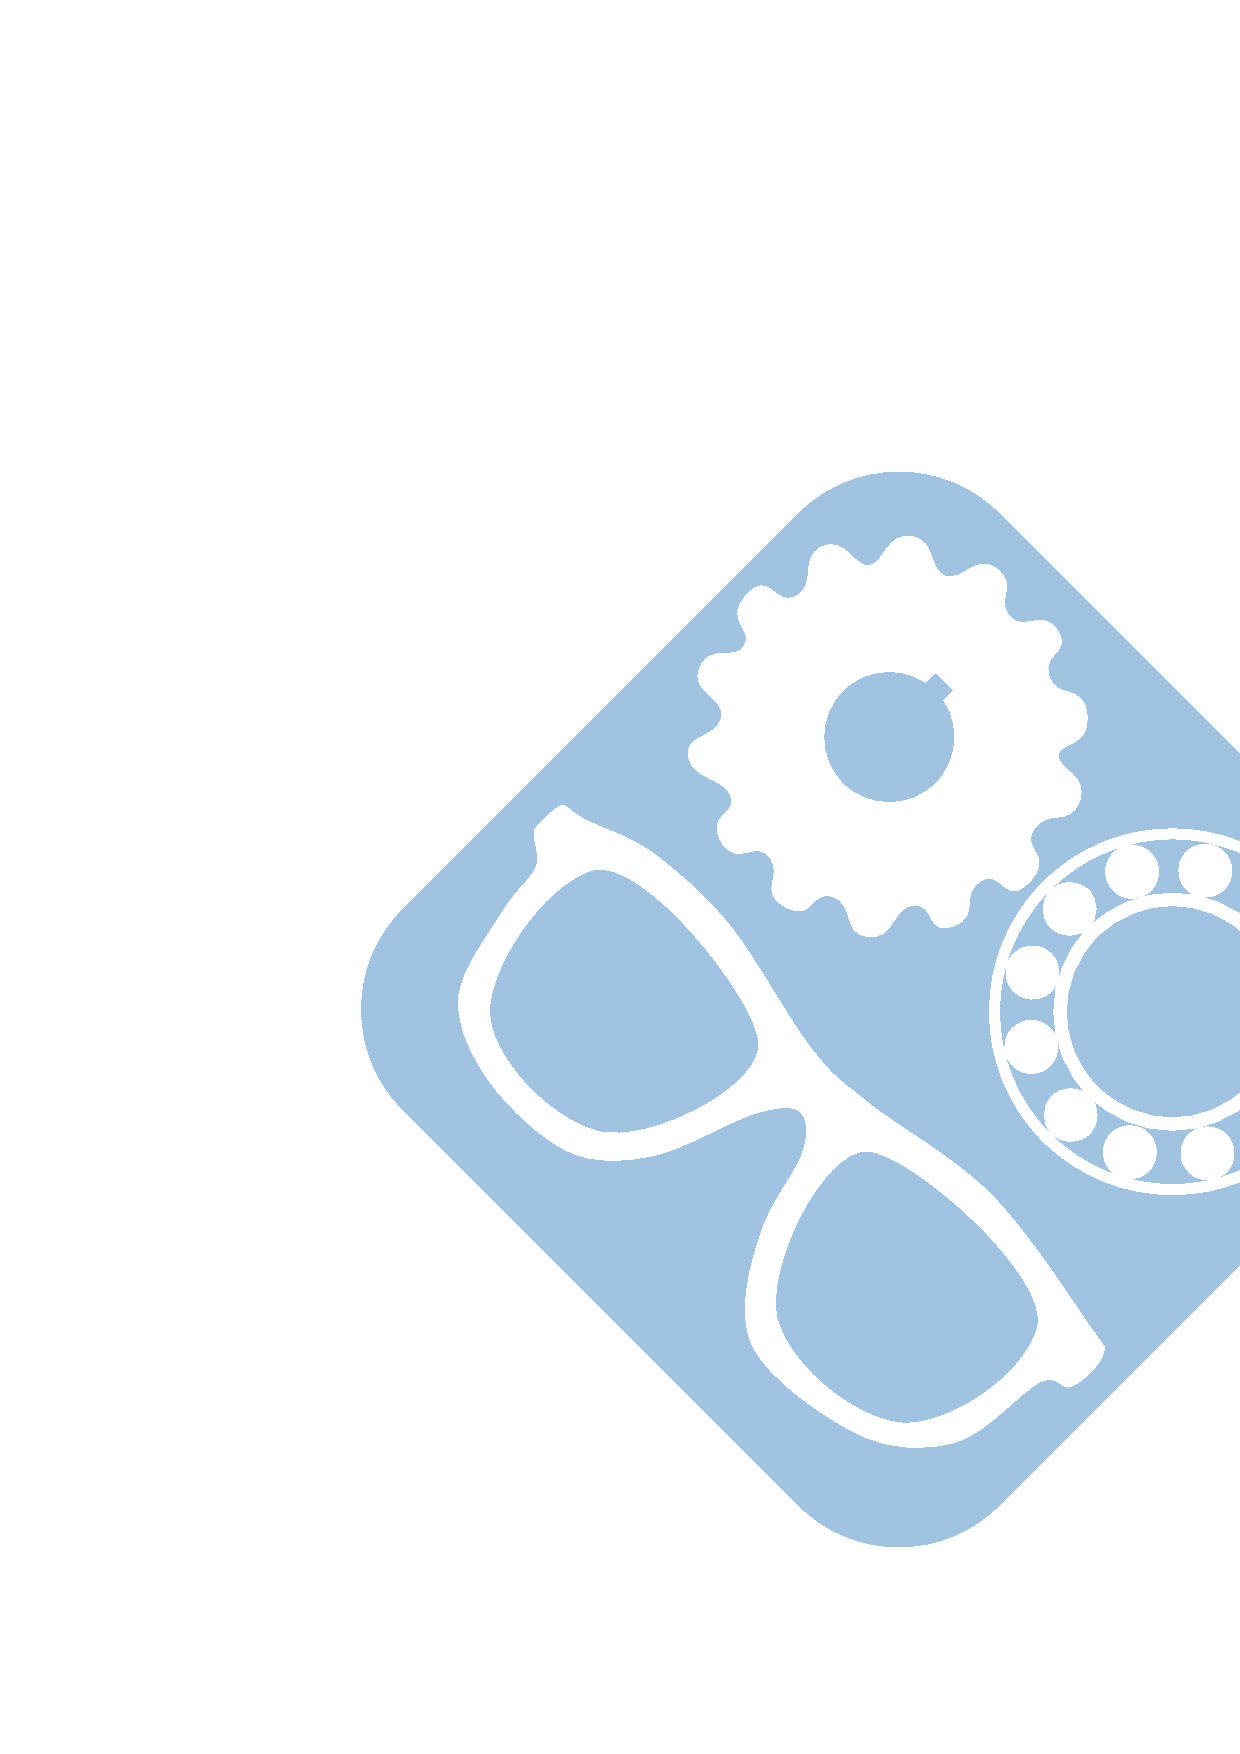
\includegraphics[width=\paperwidth,height=\paperheight,%
keepaspectratio]{../../../img/fond3}%
\end{center}
\vfill
}}}

\newcommand{\BackgroundPicdeux}{%
\put(25,-30){%
\parbox[b][\paperheight]{\paperwidth}{%
\vfill
\begin{center}
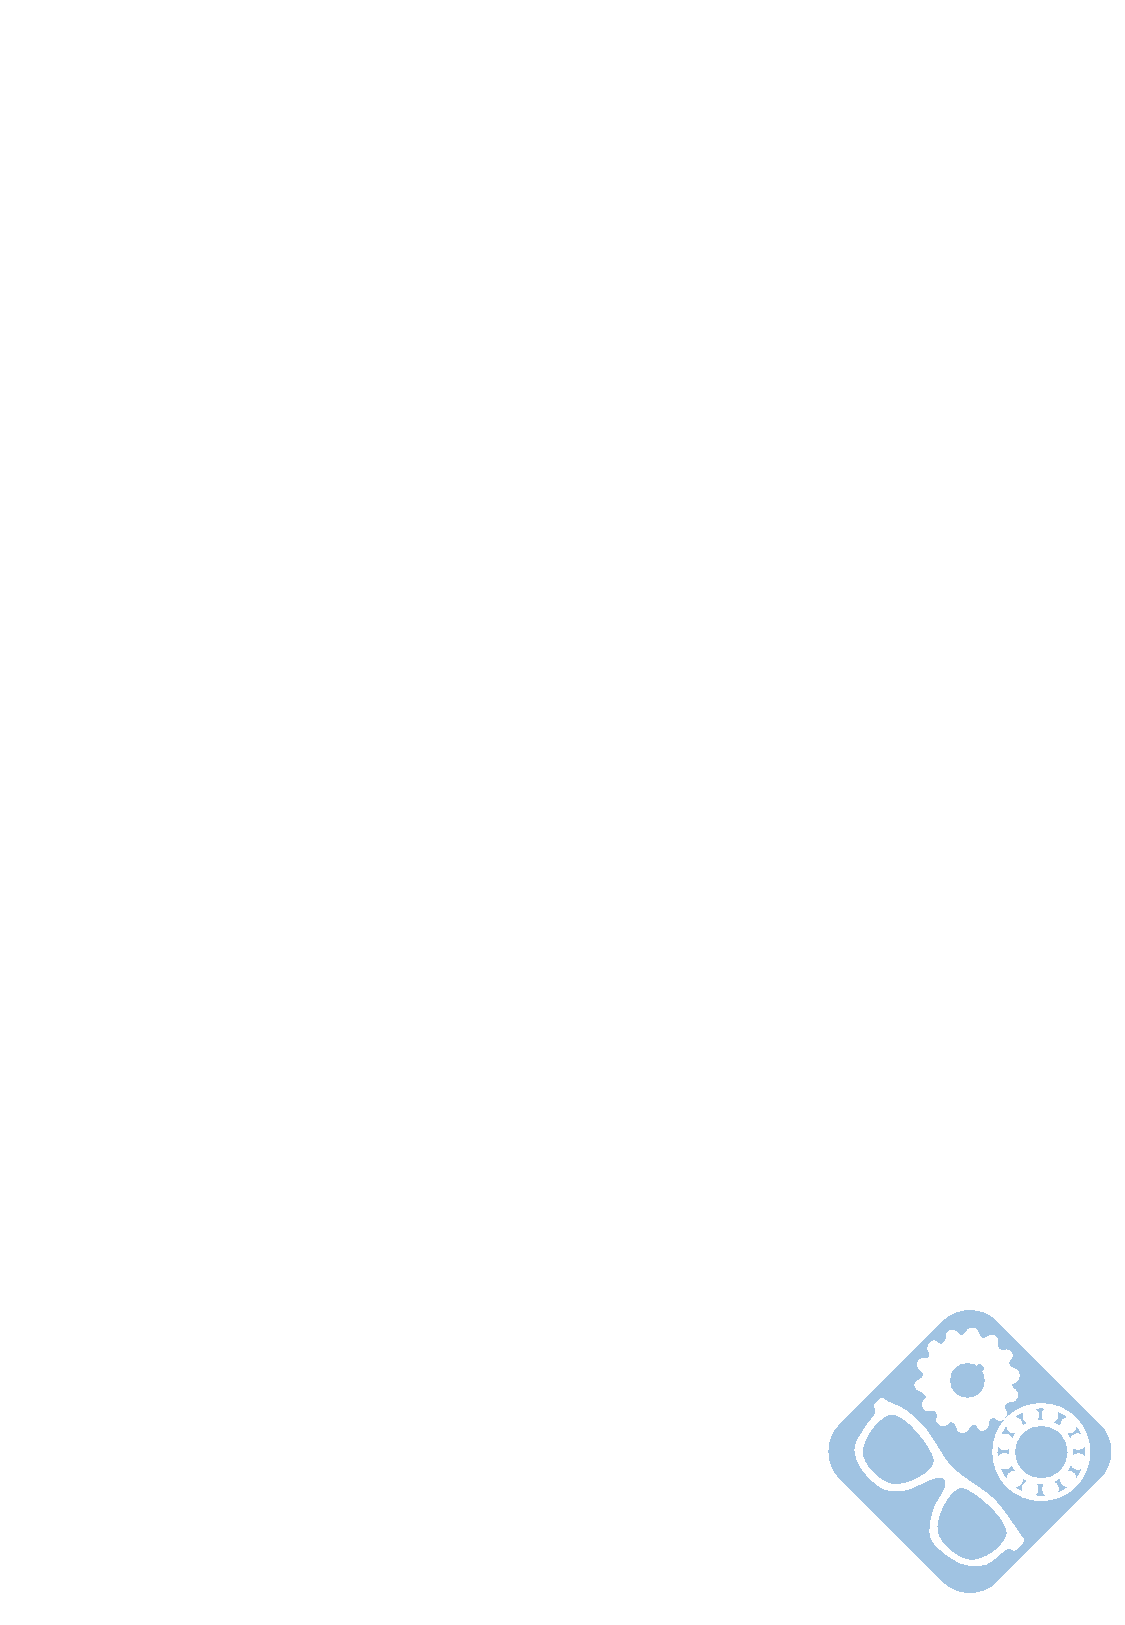
\includegraphics[width=\paperwidth,height=\paperheight,%
keepaspectratio]{../../../img/fond4}%
\end{center}
\vfill
}}}

\begin{document}

\pagestyle{empty}

\AddToShipoutPicture*{\BackgroundPic}


\includegraphics[width=2cm]{../../../img/logo}

\Huge{DS \numero - \sujet}

\vspace{1cm}

\ifdef{\prive}{\begin{center}\colorbox{danger}{\Huge{Avec Correction}}\end{center}}{}

\begin{center}
\centering\huge{PTSI}
\end{center}

\vspace{2cm}


\begin{center}
\centering\Large{\jour}
\end{center}

\vspace{2cm}

\normalsize

\tableofcontents

\newpage

\AddToShipoutPicture{\BackgroundPicdeux}

\pagestyle{fancy}

\begin{center}
\Huge \sujet
\end{center}


\normalsize


\section{Présentation}

\begin{wrapfigure}[18]{r}{0.45\textwidth}
	\vspace{-1.8cm}
  \begin{center}
    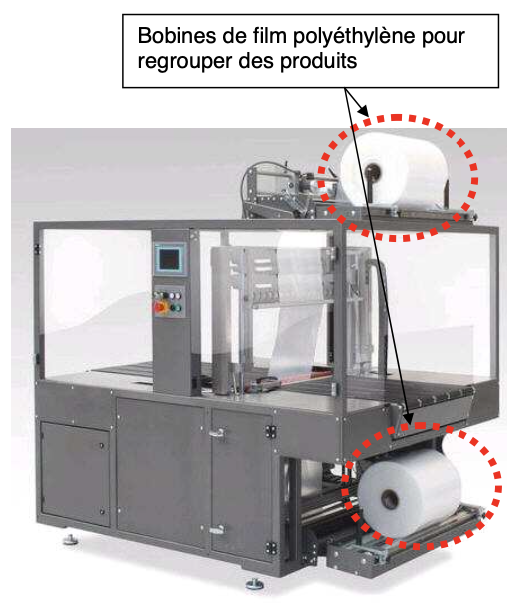
\includegraphics[width=0.4\textwidth]{img/fig01}
  \end{center}
  \caption{Mise en situation}
\label{fig01}
\end{wrapfigure}

Les productions étant automatisées dans différents secteurs (imprimerie, cosmétique, agro-alimentaire..), les opérations sur le produit fabriqué étant réalisées par les machines, il reste aux opérateurs à approvisionner les matières premières.

La fréquence des efforts est réduite mais pour obtenir une autonomie des machines suffisante, certaines fournitures sont lourdes à manipuler et cela dans un espace difficilement accessible. 

Pour les machines consommant des films (étiquettes, plastique pour regrouper des produits, cellophanage de produit unitaire (exemple parfumerie)), les bobines doivent être posées souvent en hauteur ou au ras du sol. 

Dans une démarche permettant de limiter les risques liés à la manipulation de charges lourdes, on souhaite mettre en place un système de préhension de bobines.

~\

La société TECADIS propose un chariot permettant de manipuler des bobines. 
Une option permet de basculer les bobines. Cette adaptation associée au chariot permet à l'opérateur : 
\begin{itemize}
 \item de saisir la bobine à la main sans risque,
 \item de la faire passer de la position verticale (livraison sur palette permettant de grande charge sans abimer la bobine) à la position horizontale (rotation de 90°),
 \item de la positionner au poste d'utilisation (hauteur variable),
 \item d'éviter les efforts importants dans des positions incommodantes pour l'opérateur. 
\end{itemize}

\newpage

\begin{figure}[ht]
  \begin{center}
    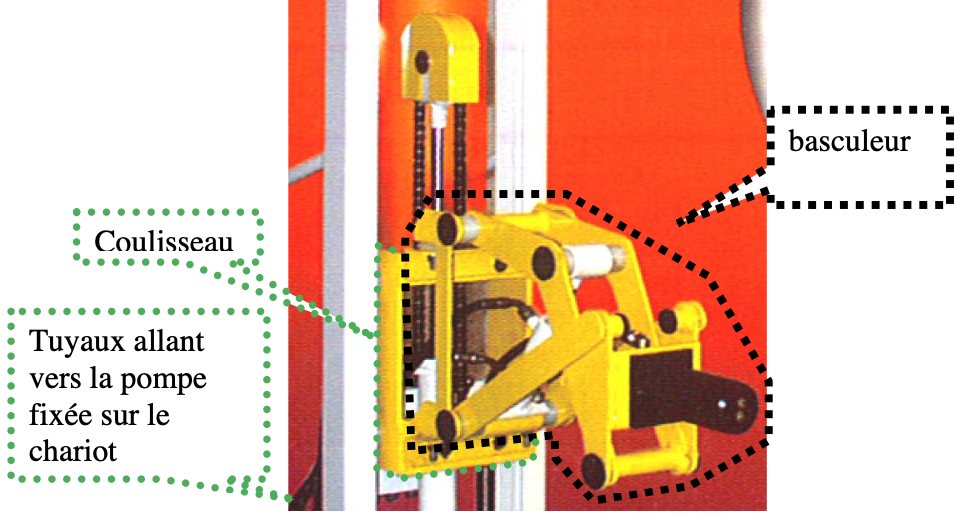
\includegraphics[width=0.8\textwidth]{img/fig02}
  \end{center}
  \caption{Principe de fonctionnement}
\label{fig02}
\end{figure}

Le basculeur s'adapte physiquement sur le coulisseau du chariot grâce à 4 perçages.

Ensuite on relie les flexibles hydrauliques aux distributeurs situés en aval d'une pompe hydraulique.

Un limiteur de pression délivre un maximum $p_{maxi}=7\;MPa$
($1\;bar=10^5Pa=0,1\;MPa=1N.mm^2$).

~\

\begin{wrapfigure}[3]{r}{0.65\textwidth}
	\vspace{-1cm}
  \begin{center}
    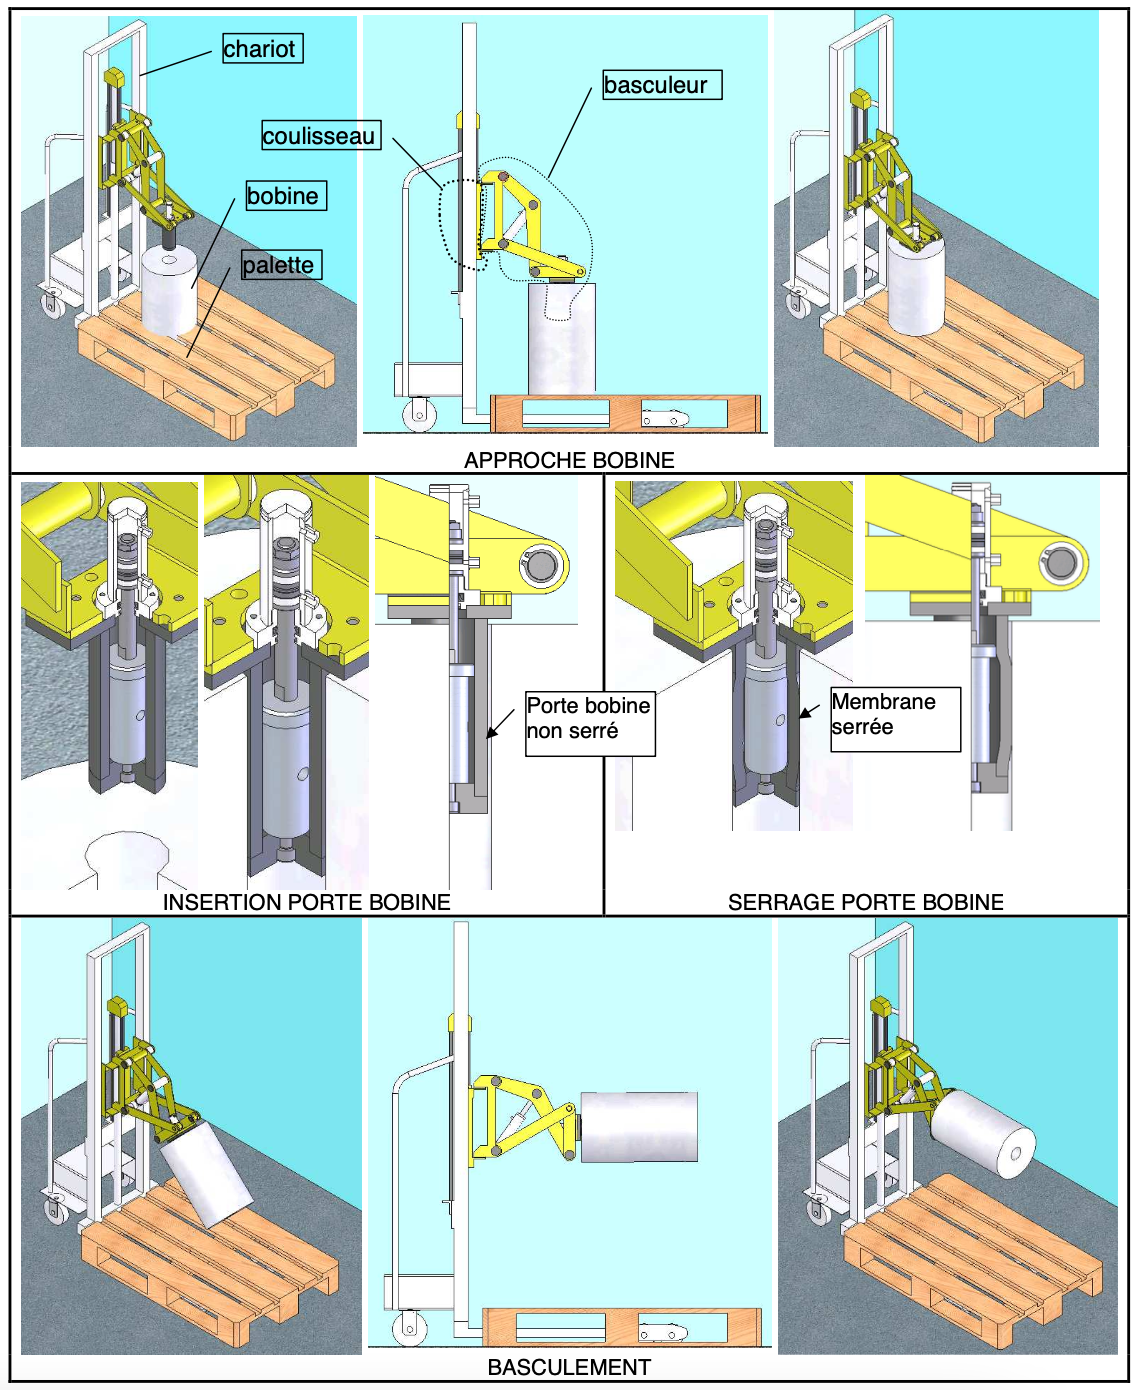
\includegraphics[width=0.5\textwidth]{img/fig03}
  \end{center}
\caption{Vue en perspective chariot basculeur}
\label{fig03}
\end{wrapfigure}

L'opérateur choisit les mouvements du basculeur avec 3 distributeurs, il ne peut faire qu'un seul mouvement à la fois : 
\begin{itemize}
 \item Montée-descente coulisseau,
 \item Serrage-desserrage mandrin,
 \item Basculement haut-bas.
\end{itemize}

\newpage

\begin{figure}[ht!]
\begin{minipage}{0.45\linewidth}
\begin{center}
 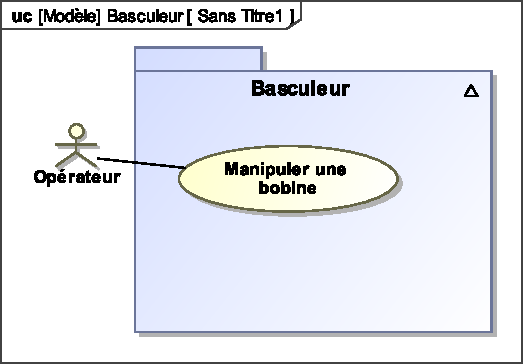
\includegraphics[width=0.9\linewidth]{img/fig04a}
\end{center}
\caption{Analyse fonctionnelle}
\label{fig04a}
\end{minipage}
\hfill
\begin{minipage}{0.45\linewidth}
\begin{center}
 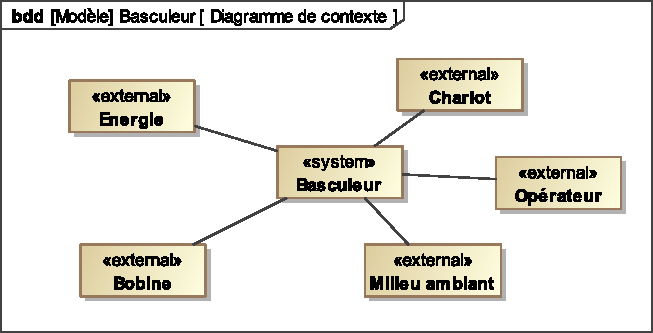
\includegraphics[width=0.9\linewidth]{img/fig04b}
\end{center}
\caption{Analyse fonctionnelle}
\label{fig04b}
\end{minipage}
\end{figure}

\begin{figure}[ht!]
\begin{center}
 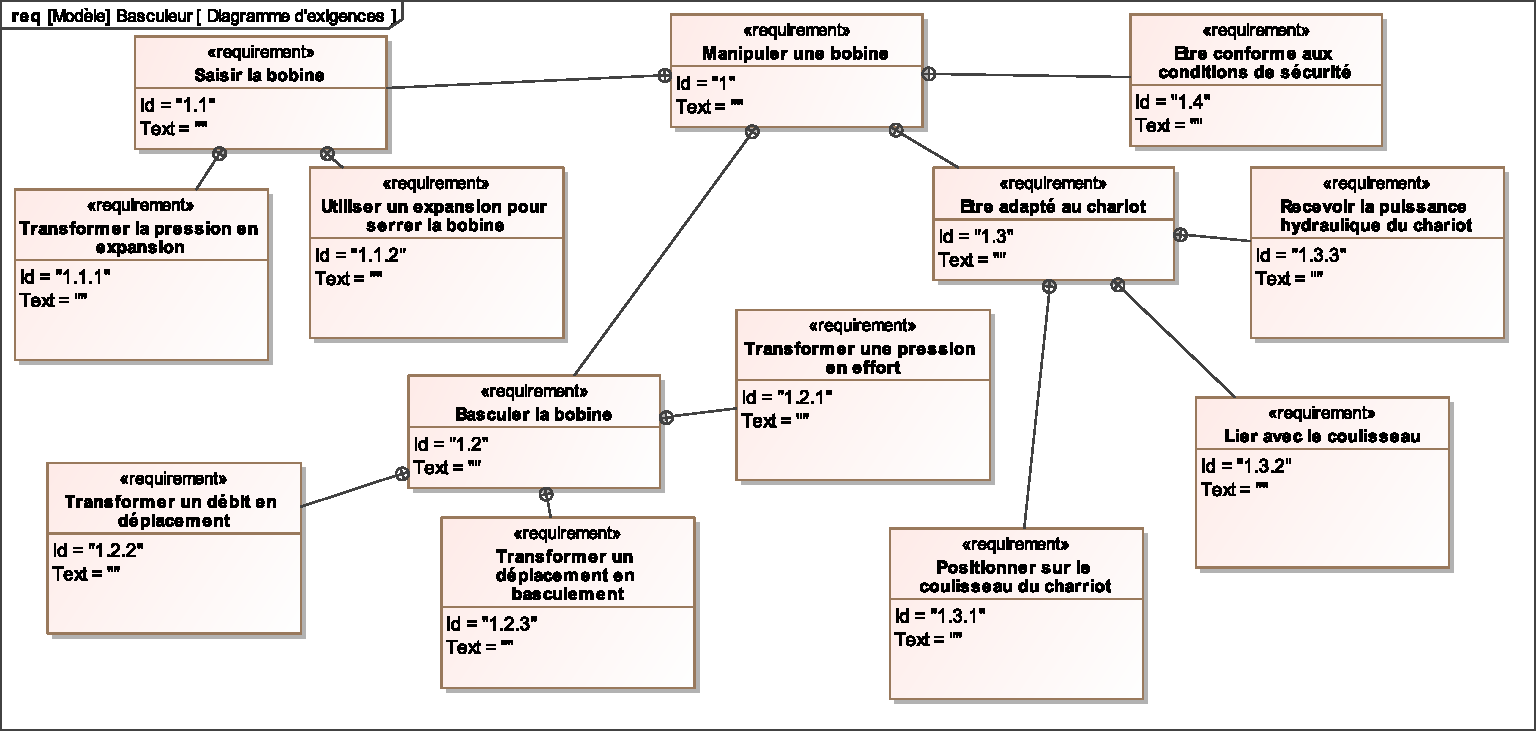
\includegraphics[width=0.8\linewidth]{img/fig04c}
\end{center}
\caption{Analyse fonctionnelle}
\label{fig04c}
\end{figure}

\begin{table}[ht!]
\begin{center}
\begin{tabular}{|m{6cm}|m{10cm}|}
\hline
Taille bobine & Longueur maxi 500 mm \\
& Longueur mini 150 mm \\
& Diamètre maxi 500 mm \\
\hline
Bobine & Diamètre intérieur 70 à 80 mm \\
\hline
Masse bobine seule & 35kg \\
\hline
Angle et vitesse de levée & De 0° (vertical) à 92° au moins, durée 8s \\
\hline
Environnement : l'appareil est utilisable dans divers secteurs & Humidité : de 100 \% à 50 \% \newline
Chaleur : stockage de -10°C à 50°C, utilisation de 5°C à 40°C \\
\hline
Durée de vie : nb de man\oe uvres & $10^6$ \\
\hline
Pression maximum & $p_{maxi}=7Mpa=70bars=7N.mm^{-2}$ \\
\hline
\end{tabular}
\end{center}
\caption{Extrait du cahier des charges}
\label{fig05}
\end{table}

\begin{wrapfigure}[12]{r}{0.5\textwidth}
\vspace{-1cm}
\begin{center}
 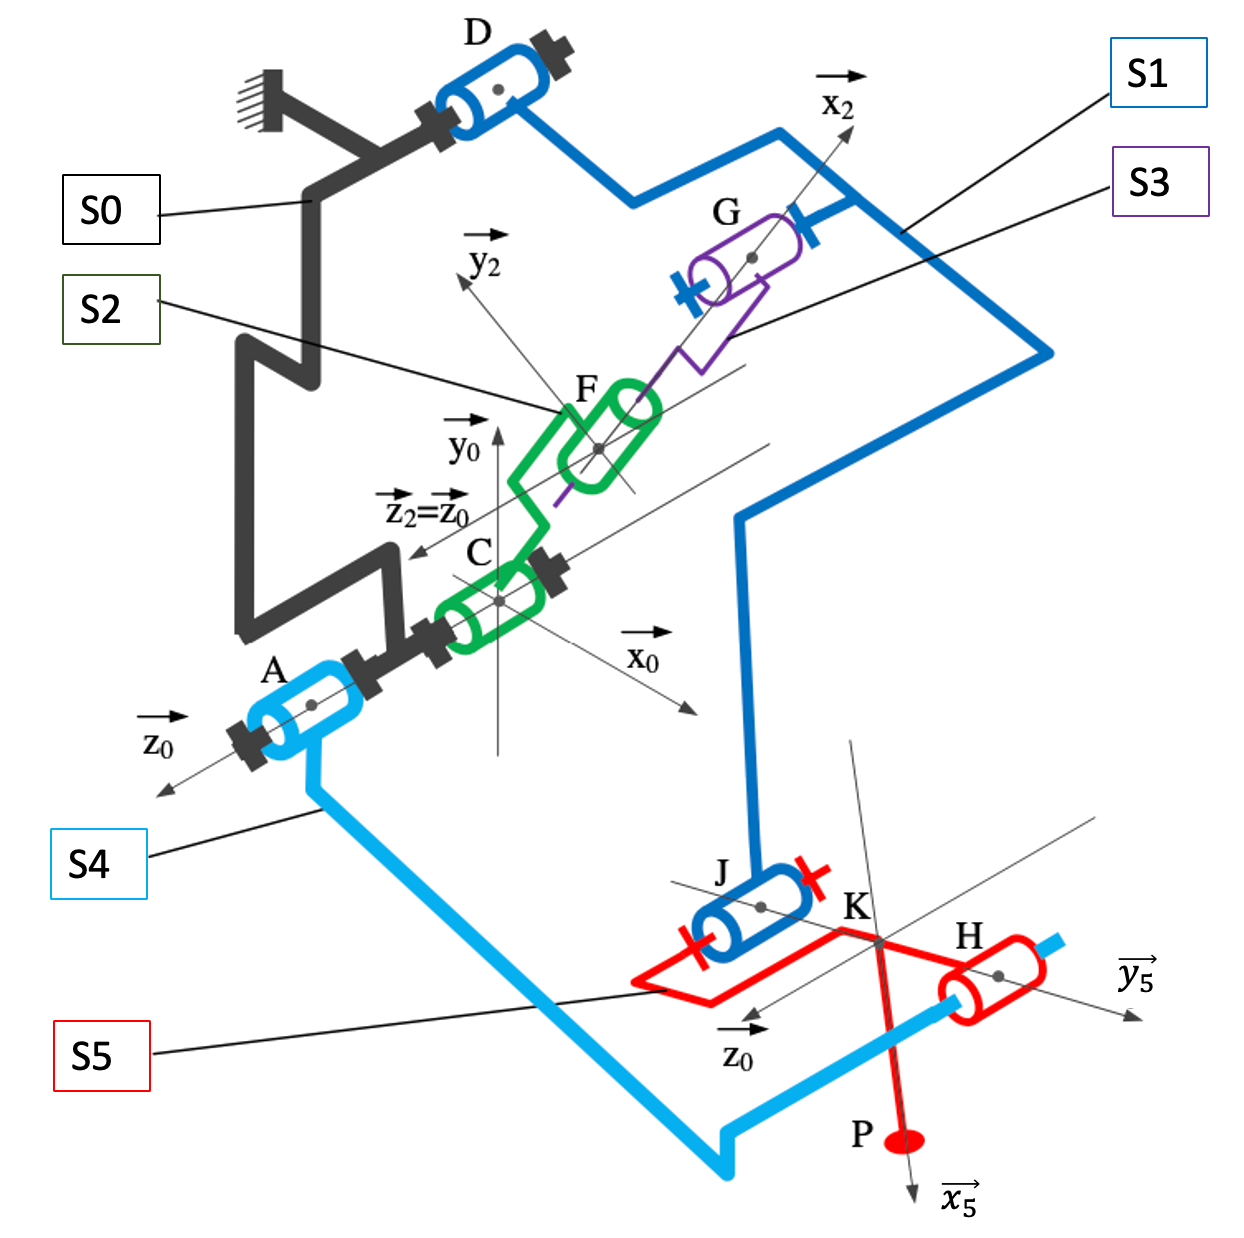
\includegraphics[width=0.9\linewidth]{img/fig06}
\end{center}
\caption{Schéma cinématique lorsque S0 est bloqué en translation}
\label{fig06}
\end{wrapfigure}

\paragraph{Paramétrage cinématique:} ~\
\begin{itemize}
 \item Repère lié au bâti S0 : \\
$R_0=(C,\overrightarrow{x_0},\overrightarrow{y_0},\overrightarrow{z_0})$
 \item Repère lié au porte-bobine S5: \\   
$R_5=(K,\overrightarrow{x_5},\overrightarrow{y_5},\overrightarrow{z_0})$
 avec \\ $\theta_5=(\overrightarrow{x_0},\overrightarrow{x_5})=(\overrightarrow{y_0},\overrightarrow{y_5})$
 \item Repère lié au fût vérin S2: \\
$R_2=(F,\overrightarrow{x_2},\overrightarrow{y_2},\overrightarrow{z_2})$ 
avec \\ $\theta_{2}=(\overrightarrow{x_0},\overrightarrow{x_2})=(\overrightarrow{y_0},\overrightarrow{y_2})$
\end{itemize}

L'axe de la bobine est donné par $(K,\overrightarrow{x_5})$:
\begin{itemize}
  \item $\theta_5=-90^{\circ}$ lorsque la bobine est en position verticale (bobine dirigée vers le bas),
  \item $\theta_5=0^{\circ}$ lorsque la bobine est en position horizontale.
\end{itemize}
~\

\paragraph{Classes d'équivalence:} ~\ \\
Le système se compose de 6 classes cinématiques équivalentes de S0 à S5:
S0 = Support, S1 = Levier, S2 = Fût vérin, S3 = Vérin mobile, S4 = Bielle, S5 = Porte bobine.

~\

\begin{minipage}[t]{0.45\linewidth}
S1 est en liaison :
\begin{itemize}
 \item pivot d'axe $(D,\overrightarrow{z_0})$ par rapport à S0,
 \item pivot d'axe $(J,\overrightarrow{z_0})$ par rapport à S5,
 \item pivot d'axe  $(G,\overrightarrow{z_0})$ par rapport à S3.
\end{itemize}

S4 est en liaison :
\begin{itemize}
 \item pivot d'axe  $(A,\overrightarrow{z_0})$ par rapport à S0,
 \item pivot glissant d'axe  $(H,\overrightarrow{z_0})$ par rapport à S5.
\end{itemize}
\end{minipage}\hfill
\begin{minipage}[t]{0.45\linewidth}
S2 est en liaison :
\begin{itemize}
 \item pivot d'axe $(C,\overrightarrow{z_0})$ par rapport à S0,
 \item pivot glissant d'axe $(C,\overrightarrow{x_2})$ par rapport à S3.
\end{itemize}
\end{minipage}

\paragraph{Dimensions utiles:} ~\
\begin{itemize}
 \item $\overrightarrow{AD}.\overrightarrow{y_0}=\overrightarrow{CD}.\overrightarrow{y_0}=a$ avec $a=160\;mm$,
 \item $\overrightarrow{JH}=b.\overrightarrow{y_0}$ avec $b=100\;mm$,
 \item $\overrightarrow{AH}\cdot \overrightarrow{y_5}=c$ avec $c=200\;mm$,
 \item $\overrightarrow{CG}=\lambda(t)\cdot\overrightarrow{x_2}$,
 \item $\overrightarrow{CA}=b.\overrightarrow{z_0}$.
\end{itemize}


\paragraph{Notations:} ~\ \\
\begin{minipage}[t]{0.45\linewidth}
Torseur cinématique:

$\left \{V_{i/ j}\right \}=\left\{
\begin{matrix}
 \overrightarrow {\Omega _{i/ j}} \\ 
 \overrightarrow {V_{M,i/j}} 
\end{matrix}
\right\}_{M}=\left\{
\begin{matrix}
 \omega_{x,ij} & {V_x }_{M,ij} \\
 \omega_{y,ij} & {V_y }_{M,ij} \\
 \omega_{z,ij} & {V_z}_{M,ij} 
\end{matrix}
\right\}_{M,B_0}$
\end{minipage}\hfill
\begin{minipage}[t]{0.45\linewidth}
Torseur des actions mécaniques:

$\left \{T_{i\rightarrow j}\right \}=\left\{
\begin{matrix}
 \overrightarrow {F_{i\rightarrow j}} \\ 
 \overrightarrow {M_{M,i\rightarrow j}} 
\end{matrix}
\right\}_{M}=\left \{
\begin{matrix}
 X_{ij} & {L }_{M,ij} \\
 Y_{ij} & {M }_{M,ij} \\
 Z_{ij} & {N }_{M,ij} 
\end{matrix}
\right \}_{M,B_0}$
\end{minipage}

\section{Etude de l'asservissement en position selon $\vec{y_0}$ du système de basculement}

Pour positionner le coulisseau (solidaire du système basculeur) selon la direction $\overrightarrow{y_0}$ , on utilise un vérin hydraulique.

\question{Compléter l'extrait du schéma organique Chaîne d'Information-Chaîne d'Energie-Puissance en nommant les éléments réalisant les fonctions Alimenter, Moduler et Convertir. Préciser les énergies entrantes et sortantes des 3 blocs fonction.}

\paragraph{Hypothèse:} Le fluide présent dans le vérin hydraulique est incompressible.

\paragraph{Données:} ~\
\begin{itemize}
 \item débit volumique: $q(t)$ en $m^3.s^{-1}$,
 \item déplacement du tiroir de la servocommande: $x(t)$ en $m$,
 \item déplacement de la tige qui se déplace: $z(t)$ en $m$,
 \item débit par fuite entre les 2 chambres de la servocommande: $q_P(t)$ en $m^3.s^{-1}$,
 \item différence de pression entre les 2 chambres du vérin: $\Delta_P$ en $N.mm^{-2}$,
 \item masse de l'ensemble coulisseau+système de basculeur: $M$ en $kg$.
\end{itemize}

\paragraph{Équations:} ~\
\begin{itemize}
 \item Comportement de la servocommande: $q(t)=k\cdot x(t)$ (1)
 \item Comportement du vérin: $q(t)=S\cdot \dot {z}(t)+q_P(t)$ (2)
 \item $q_P(t)=f\cdot \Delta_P(t)$ (3) ou  $f$ est un coefficient constant.
 \item $F(t)=S\cdot \Delta_P(t)$ (4)
 \item Comportement de la masse: $F(t)=M\cdot \ddot{z}(t)$ (5)
\end{itemize}

\paragraph{Remarque:} on notera $L[x(t)]=X(p)$, $L[z(t)]=Z(p)$, $L[q(t)]=Q(p)$, $L[q_P(t)]=Q_P(p)$, $L[\Delta_P(t)]=\Delta_P(p)$, $L[F(t)]=F(p)$.

\question{Transformer les équations précédentes données dans le domaine de Laplace (conditions initiales nulles).}

\question{Compléter alors le schéma bloc correspondant au comportement de la servocommande.}

\question{Exprimer la fonction de transfert $H_{BO}=\frac{Q_P(p)}{\epsilon_Q(p)}$ puis exprimer $H_1(p)=\frac{Z(p)}{Q(p)}$.}

\question{En déduire la fonction de transfert en boucle fermée  $H_2(p)=\frac{Z(p)}{X(p)}$. Mettre $H_2(p)$ sous forme canonique. Indiquez la classe, l'ordre, le gain et les caractéristiques de l'ordre trouvé. Faire l'application numérique et préciser les unités en unité SI de base.}

\newpage

Pour compléter l'étude, on donne les valeurs numériques suivantes:
\begin{itemize}
 \item $S=3000\;mm^2$,
 \item $f=6\;dm^3\cdot min^{-1}\cdot MPa^{-1}$,
 \item $k=0,24\;m^3\cdot s^{-1}\cdot mm^{-1}$,
 \item $M=42\;kg$.
\end{itemize}

\question{Tracer le diagramme de Bode asymptotique en gain et en phase de cette fonction de transfert en boucle fermée, en précisant les pulsations de coupure lorsque c'est nécessaire.}


\section{Analyse et compréhension du système de basculement}

On étudie maintenant le système de basculement, le chariot est alors bloqué en translation (pas de mouvement suivant $\vec{z}$ de S0).

\question{En s'aidant de l'extrait du dessin d'ensemble du système de basculement de la figure \ref{fig08} (le format original A3 a été réduit, mais cela n'impacte pas vos réponses) et de la nomenclature figure \ref{fig09}, indiquer l'ensemble des pièces constituant la classe d'équivalence S3 VERIN MOBILE. La pièce 29 est supposée fixe par rapport au LEVIER N°4.}

\question{Compléter le graphe des liaisons du système étudié.}

\question{Décrire la nature du mouvement d'entrée de ce système.}

\question{Décrire la nature du mouvement de sortie de ce système. En déduire la mobilité utile de ce système.}

\question{Compléter le tableau en indiquant les 6 composantes des torseurs cinématique et statique des différentes liaisons. (Attention, il faut bien respecter les notations de l'énoncé). L'exemple de la liaison entre S0 et S4 est fourni.}

\question{En écrivant la relation littérale utilisée, donner le degré d'hyperstatisme du système (S0, S1, S2, S3, S4, S5).}

\question{En considérant uniquement la chaîne {0-2-3-1}, écrire une fermeture cinématique à l'aide des torseurs des différentes liaisons, au point A et dans la base $(\overrightarrow{x_2},\overrightarrow{y_2},\overrightarrow{z_2}=\overrightarrow{z_0})$.}

\question{En utilisant la relation liant inconnues cinématiques, rang des équations (nombre d'équations indépendantes) et mobilité, donner la mobilité $m$ de cette chaîne.}

\newpage

\section{Étude de la fonction \og Basculer la bobine \fg}

\paragraph{Hypothèse:} ~\ 
\begin{itemize}
 \item L'étude des mouvements et des trajectoires s'effectuera dans le plan médian du basculeur $(A,\overrightarrow{x_0},\overrightarrow{y_0})$,
 \item L'étude sera réalisée dans 3 positions : celles-ci sont superposées sur le document réponse question \ref{q15} : La position 1 verticale de la bobine $(\theta_5=0^{\circ})$ , la position 2 inclinée $(\theta_5=-45^{\circ})$ et la position finale 3 $(\theta_5=-90^{\circ})$,
 \item Dans les positions 1 et 3 les vitesses sont nulles (début et fin de mouvement), la vitesse maximum du vérin est atteinte lors de la position intermédiaire 2. Sur le document réponse question \label{q16}, seule la position 2 est donnée,
 \item Les liaisons sont simplifiées : en A, D, G, J, H les liaisons sont toutes des liaisons pivot.
\end{itemize}

On donne le schéma cinématique plan suivant:

\begin{figure}[ht!]
\begin{center}
 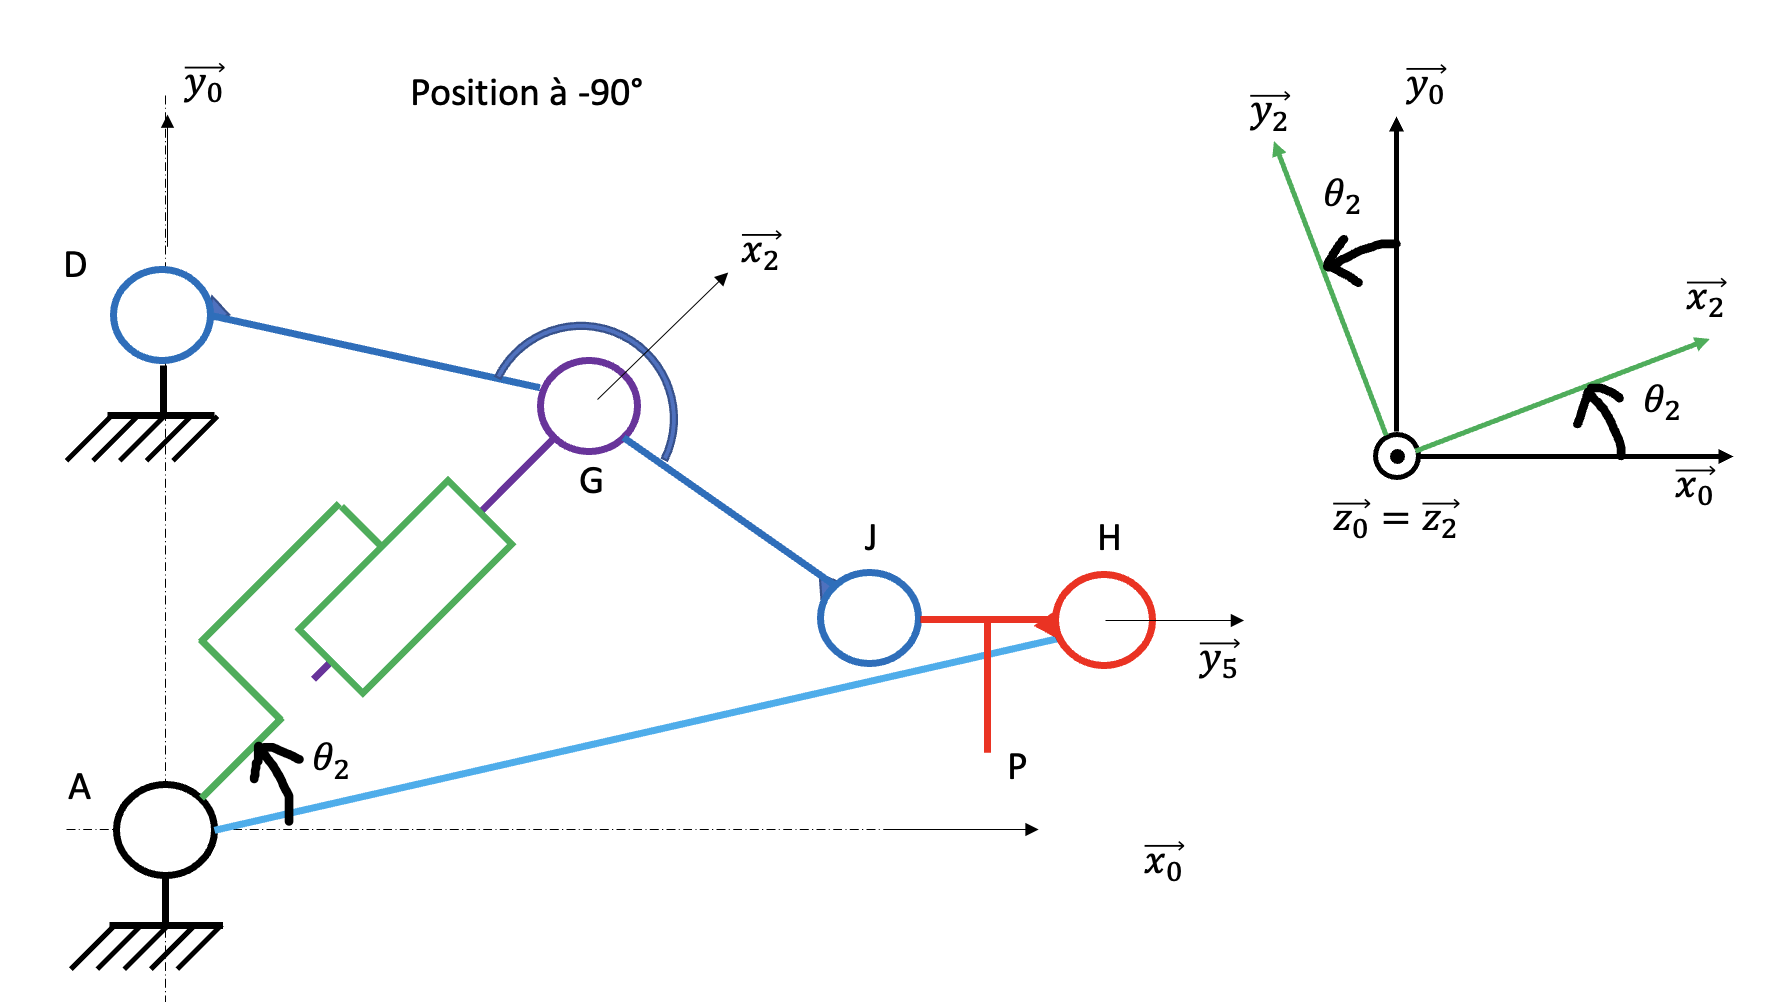
\includegraphics[width=0.7\linewidth]{img/fig07}
\end{center}
\caption{Schéma cinématique}
\label{fig07}
\end{figure}

\paragraph{Course de l'actionneur} ~\ \\
Le vérin choisi par le constructeur a une course maximale de $C_m=100\;mm$.
Sur les documents réponses fournis, l'échelle des distances peut être obtenue connaissant la dimension entre A et D (cf. paramétrage).

\question{En se basant sur les points fournis sur le document réponse, écrire l'expression littérale de la course utile $C_u$ et faire l'application numérique. Conclure sur la compatibilité de la course du vérin $C_u$ et la course utile du vérin choisi.\label{q15}}

\paragraph{Sécurité de la bobine} ~\ \\
La bobine manipulée est entourée d'un film plastique de protection.

Le point Q1 est un point de contact entre le sol et la bobine, il appartient à la classe cinématique S5. Le point M1 est également un point de contact entre la bobine et le sol situé côté support.

\question{A partir de la trajectoire des points J et H, déduire la position du $CIR_{50}$. Tracer alors la direction et le sens du vecteur vitesse $\overrightarrow{V_{Q1 \in S_5/S_0}}$. (on ne demande pas la norme). Tracer également  la direction et le sens du vecteur vitesse $\overrightarrow{V_{M1 \in S_5/S_0}}$.\label{q16}}

\question{Que risque la bobine en contact avec le sol au début du mouvement? Si le diamètre extérieur de la bobine est encore plus grand que celui représenté sur le système actuel, que risque-t-il d'arriver au début du mouvement? Quelle précaution l'utilisateur devra prendre pour pallier le problème?}

\paragraph{Vitesse et sécurité pour l'utilisateur} ~\ \\

En position 2, la tige du vérin est à sa vitesse maximum de sortie. On peut vérifier, pour des raisons de précautions, que la vitesse maximum en bout de bobine n'atteigne pas la vitesse limite $\left\|\overrightarrow{V_{N,S5/S0}} \right\|=\;200\;mm.s^{-1}$. Le point N est un point à l'extrémité de la bobine en position 2.

Les réponses aux questions suivantes se feront sur le même document réponse de la question 19, qui contient 2 épures A et B avec des échelles différentes.

\question{Tracer sur l'épure A le vecteur de sortie de tige du vérin $\overrightarrow{V_{G,S2/S3}}$ , sa norme vaut $\left\|\overrightarrow{V_{G2,S2/S3}}\right\|=\;11\;mm.s^{-1}$.}

\question{Écrire la composition de vitesse permettant d'obtenir $\overrightarrow{V_{G2,S1/S0}}$. 
Justifier la valeur de $\overrightarrow{V_{G2,S1/S3}}$. Tracer toutes les directions des vitesses de cette expression obtenues sur l'épure A.}

\question{En déduire et tracer $\overrightarrow{V_{G2,S1/S0}}$ sur l'épure A.}

! ATTENTION, les tracés se font maintenant sur l'épure B !

\question{Reporter $\overrightarrow{V_{G2,S1/S0}}$ en utilisant l'échelle de l'épure B.}

\question{Tracer $\overrightarrow{V_{J2,S1/S0}}$ en citant la méthode utilisé. Vous ferez apparaître vos tracés.}

\question{Après avoir justifier la valeur de $\overrightarrow{V_{J2,S5/S1}}$, exprimer $\overrightarrow{V_{J2,S5/S0}}$ en utilisant une composition de vitesse.}

\question{Après avoir justifier la valeur de  $\overrightarrow{V_{H2,S5/S4}}$, donner la direction de $\overrightarrow{V_{H2,S5/S0}}$ sur l'épure B.}

\question{D'après les question 24 et 25, trouver le CIR du mouvement de S5 par rapport à S0 et tracer le vecteur $\overrightarrow{V_{H2,S5/S0}}$ sur l'épure B.}

\question{Avec la méthode de votre choix, et en justifiant vos tracés, tracer sur l'épure B  $\overrightarrow{V_{N,S5/S0}}$. Donner la valeur de la norme de $\overrightarrow{V_{N,S5/S0}}$.}

\question{Conclure par rapport au cahier des charges donné en début de partie.}

\newpage

\section{Lecture de plan}

\question{Colorier les classes d'équivalence directement sur le document A3.}

\question{Dessiner un graphe de liaison.}

\question{Représenter le système par un schéma cinématique, dans le plan XY.}

\begin{figure}
\vspace{-0.5cm}
\begin{center}
 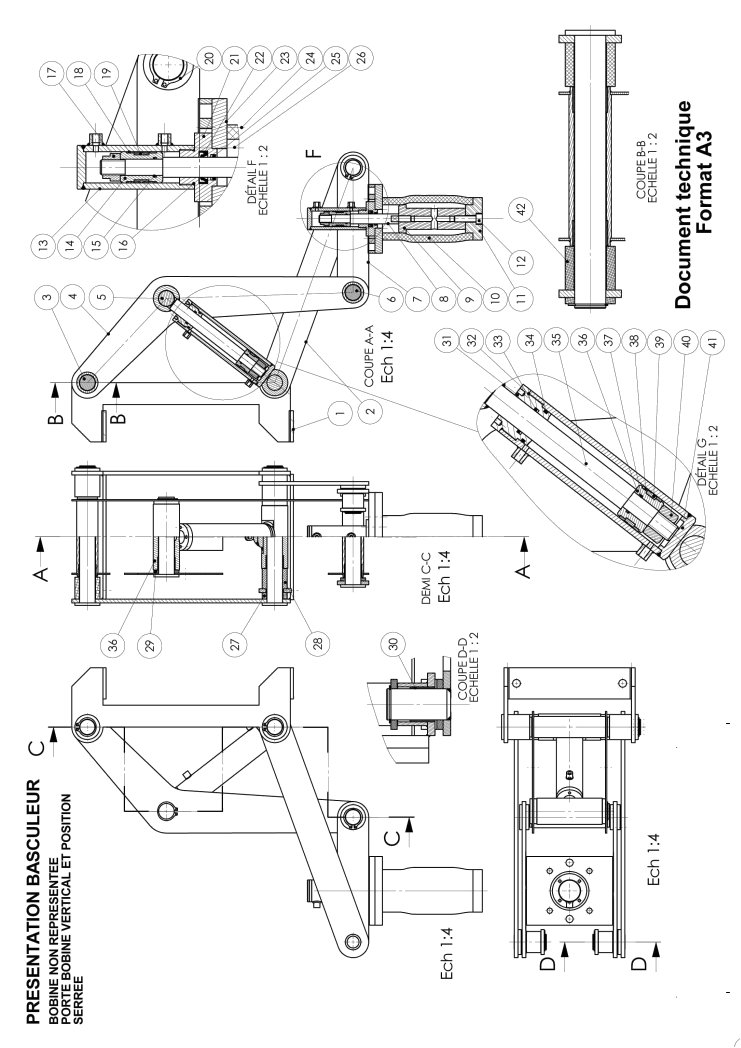
\includegraphics[width=\linewidth]{img/fig08.png}
\end{center}
\caption{Extrait du dessin d'ensemble}
\label{fig08}
\end{figure}

\begin{figure}
\begin{center}
 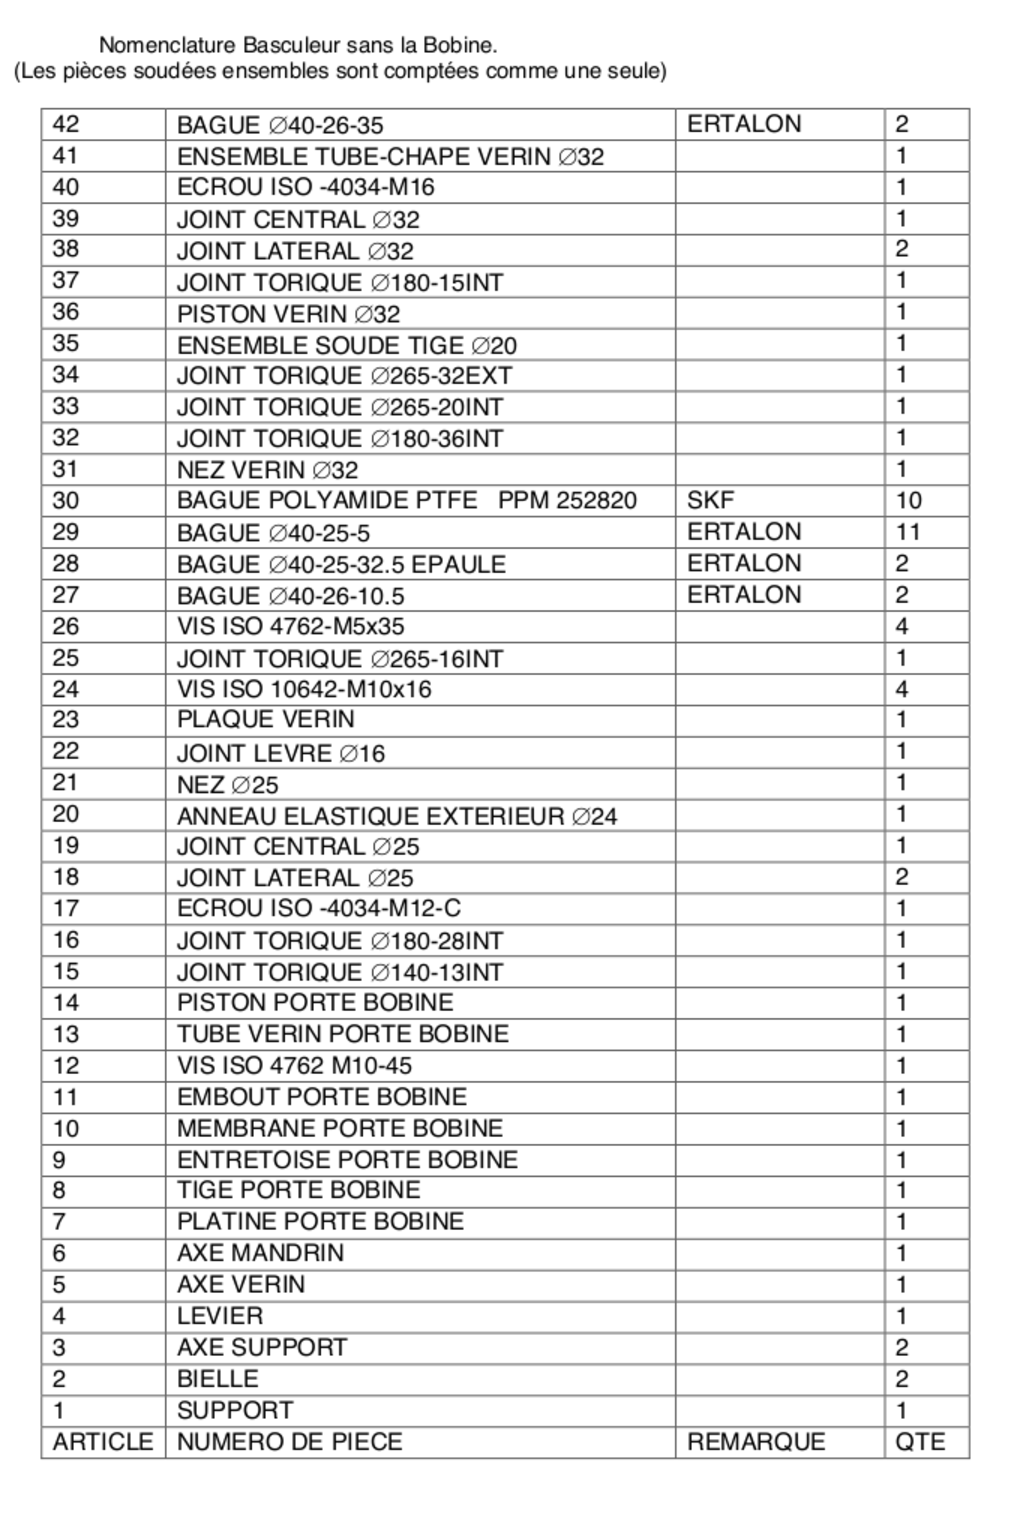
\includegraphics[width=0.8\linewidth]{img/fig09}
\end{center}
\caption{Nomenclature}
\label{fig09}
\end{figure}

\cleardoublepage

\ifdef{\public}{\pagestyle{documentreponse}}{\pagestyle{correction}}

\reponse{}{\begin{center}
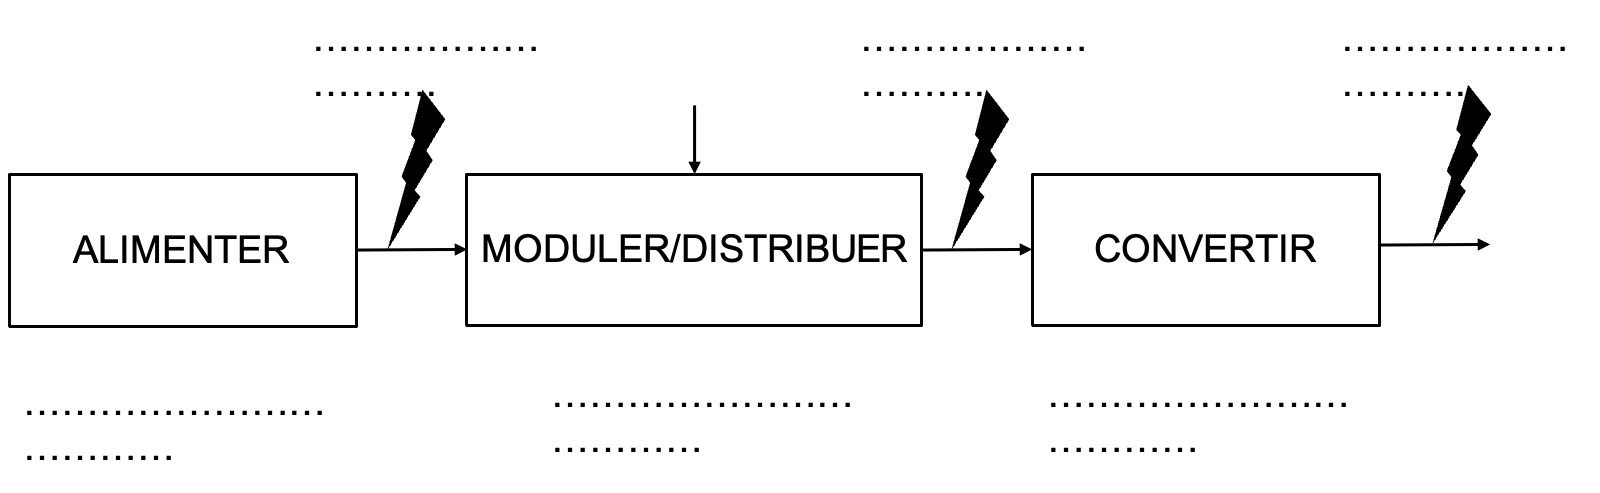
\includegraphics[width=0.9\linewidth]{img/DR01}
\end{center}}{\begin{center}
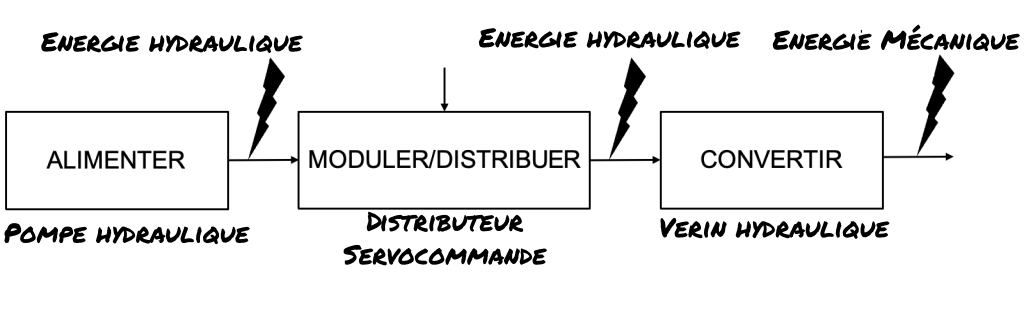
\includegraphics[width=0.9\linewidth]{img/DR01_cor}
\end{center}}

\reponse{4}{}{$Q(p)=k\cdot X(p)$, $Q(p)=S\cdot p\cdot Z(p)+Q_p[p)$, $Q_p(p)=f\cdot \Delta_p(p)$, $F(p)=S\cdot \Delta_p(p)$.}

\reponse{2}{\begin{center}
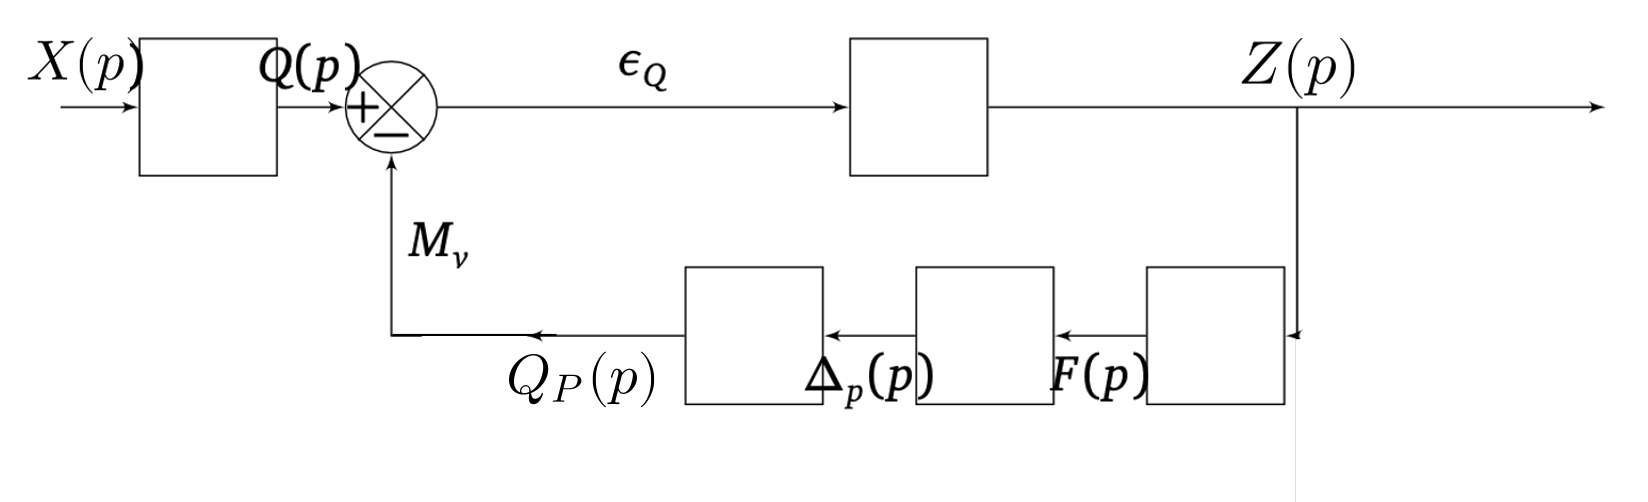
\includegraphics[width=0.9\linewidth]{img/DR02}
\end{center}}{ \begin{center}
  \def\svgwidth{0.9\linewidth}
  \input{img/DR02_cor.pdf_tex}
 \end{center}}

\reponse{9}{}{$H_{BO}=\dfrac{f\cdot M\cdot p}{S^2}$, $H_{1}=\dfrac{\dfrac{1}{S\cdot p}}{1+\dfrac{f\cdot M\cdot p}{S^2}}=\dfrac{\dfrac{1}{S}}{p\cdot \left(1+\dfrac{f\cdot M}{S^2}\cdot p\right)}$}

\reponse{9}{}{$H_{2}=\dfrac{\dfrac{k}{S}}{p\cdot \left(1+\dfrac{f\cdot M}{S^2}\cdot p\right)}$
Fonction de classe 1, d'ordre 2, gain $\dfrac{k}{S}=\dfrac{24\cdot 10^7}{3\cdot 10^3}=8\cdot 10^4\cdot s^{-1}$\\ $\tau=\dfrac{f\cdot M}{S^2}=\dfrac{6\cdot 10^{-3}\cdot 42}{60\cdot 10^6\cdot 3000^2\cdot 10^{-6}}=\dfrac{10^{-10}\cdot 42}{9}=5\cdot 10^{-10}s$.
}

\ifdef{\public}{\newpage}

\reponse{4}{\begin{center}
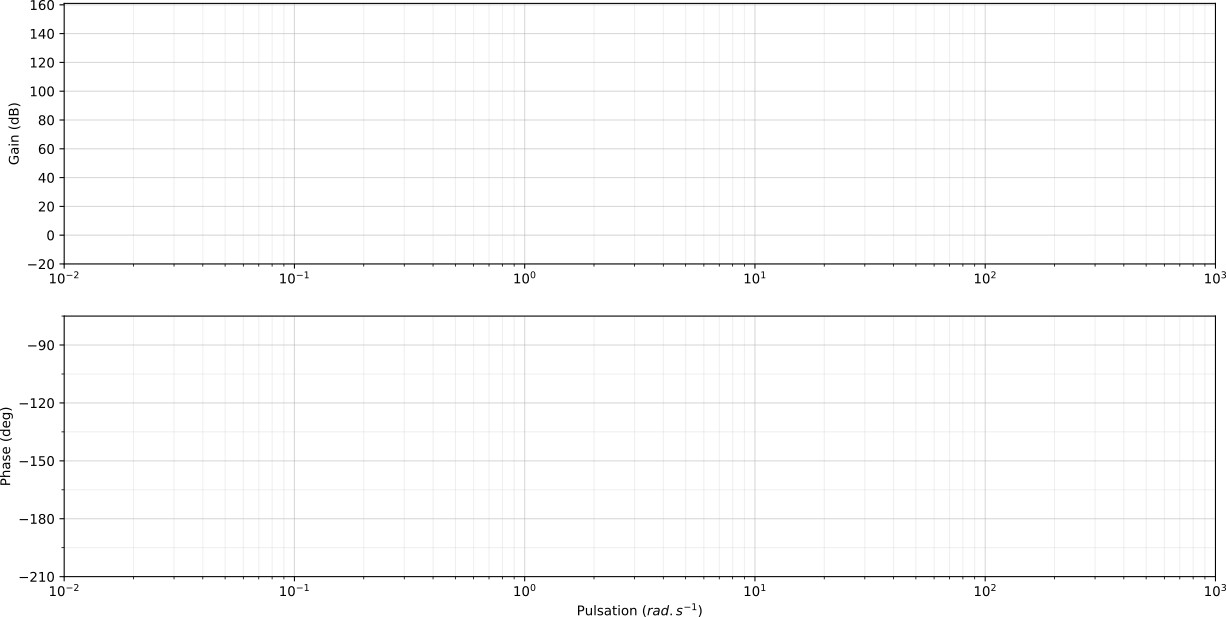
\includegraphics[width=0.9\linewidth]{img/DR03}
\end{center}}{\begin{center}
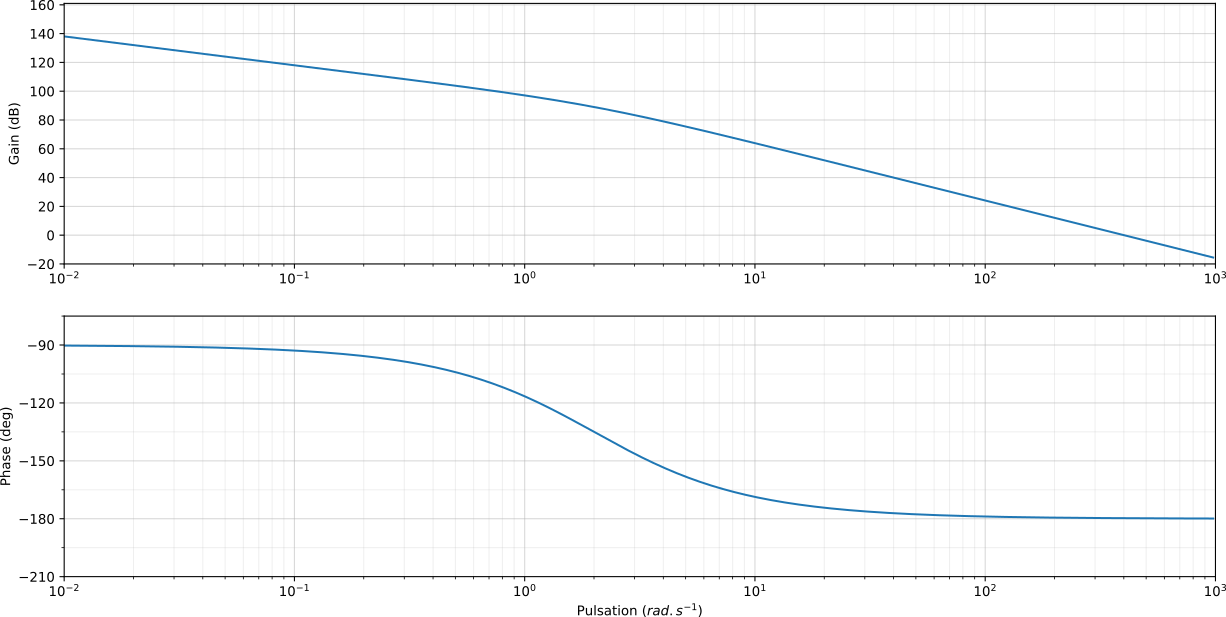
\includegraphics[width=0.9\linewidth]{img/DR03_cor}
\end{center}}

\reponse{5}{}{Classe équivalence S3 est constituée des pièces 29, 36, 37, 38, 39, 40, 41.}

\ifdef{\public}{\newpage}

\reponse{2}{\begin{center}
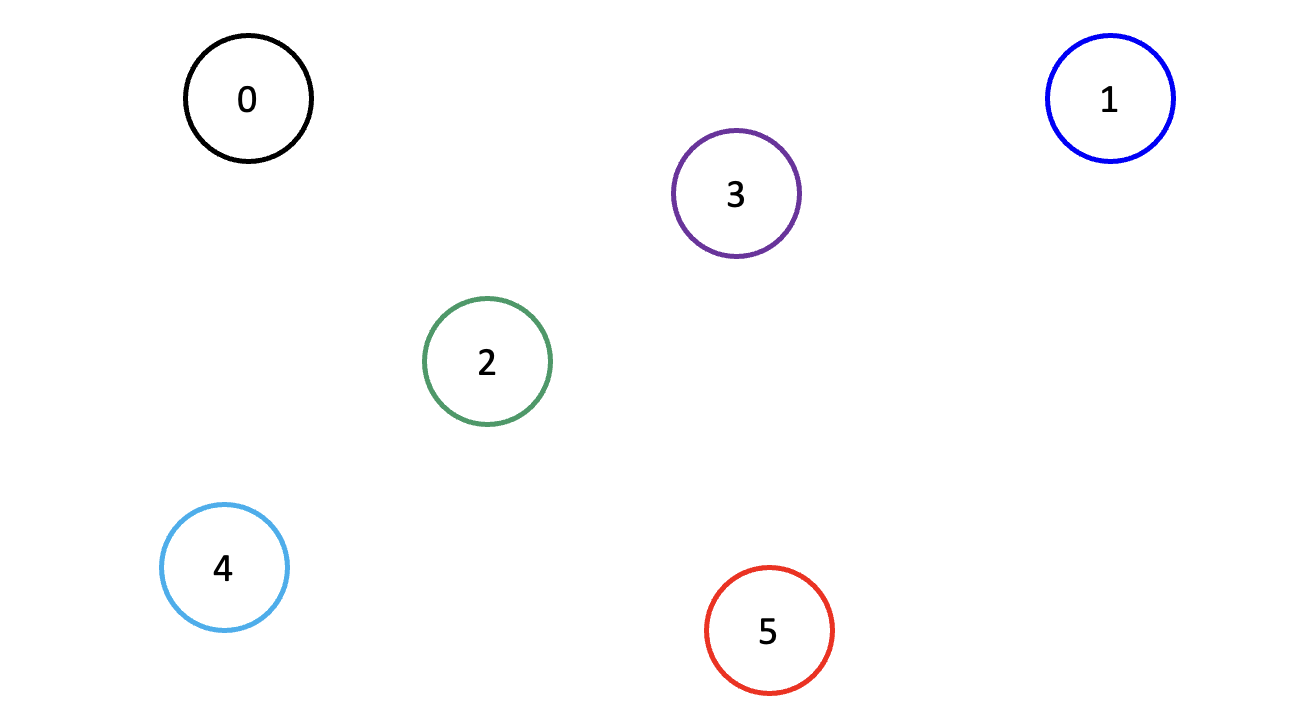
\includegraphics[width=0.9\linewidth]{img/DR04}
\end{center}}{\begin{center}
  \def\svgwidth{0.9\linewidth}
  \input{img/DR04_cor.pdf_tex}
 \end{center}}

\reponse{3}{}{Le mouvement d'entrée de ce système est la translation de S2/S3}

\reponse{3}{}{Le mouvement de sortie est une rotation de la pièce 5. Il n'y a donc qu'une seule mobilité dans ce système.}

\reponse{2}{\begin{center}
\begin{tabular}{|m{0.5cm}|m{1.7cm}|m{2cm}|m{5.8cm}|m{5.5cm}|}
\hline
Liais. & Désig & Elém. géo. & Torseur cinématique & Torseur cinématique \\ 
\hline
S0-S4 & Pivot d'axe $(A,\vec{z_0})$ & Tout point de l'axe  $(A,\vec{z_0})$ & \small$\left\{V_{S0/S4}\right\}=\left\{\begin{array}{cc}0 & 0\\0&0\\\omega_{z,04}&0\end{array}\right\}_{A,B_0}$ & \small$\left\{T_{S4\rightarrow S0}\right\}=\left\{\begin{array}{cc}X_{40} & L_{A,40}\\Y_{40}&M_{A,40}\\Z_{40}&0\end{array}\right\}_{A,B_0}$\\
\hline
S3-S1 &  &  & \small$\left\{V_{S1/S3}\right\}=\left\{\begin{array}{cc}...... & ......\\...... & ......\\...... & ......\end{array}\right\}_{.....}$ & \small$\left\{T_{S3\rightarrow S1}\right\}=\left\{\begin{array}{cc}...... & ......\\...... & ......\\...... & ......\end{array}\right\}_{.....}$\\
\hline
S1-S0 &  &  & \small$\left\{V_{S1/S0}\right\}=\left\{\begin{array}{cc}...... & ......\\...... & ......\\...... & ......\end{array}\right\}_{.....}$ & \small$\left\{T_{S0\rightarrow S1}\right\}=\left\{\begin{array}{cc}...... & ......\\...... & ......\\...... & ......\end{array}\right\}_{.....}$\\
\hline
S2-S3 &  &  & \small$\left\{V_{S2/S3}\right\}=\left\{\begin{array}{cc}...... & ......\\...... & ......\\...... & ......\end{array}\right\}_{.....}$ & \small$\left\{T_{S3\rightarrow S2}\right\}=\left\{\begin{array}{cc}...... & ......\\...... & ......\\...... & ......\end{array}\right\}_{.....}$\\
\hline
\end{tabular}
\end{center}}{\begin{center}
\begin{tabular}{|m{0.5cm}|m{1.7cm}|m{2cm}|m{5.8cm}|m{5.5cm}|}
\hline
Liais. & Désig & Elém. géo. & Torseur cinématique & Torseur cinématique \\ 
\hline
S0-S4 & Pivot d'axe $(A,\vec{z_0})$ & Tout point de l'axe  $(A,\vec{z_0})$ & \small$\left\{V_{S0/S4}\right\}=\left\{\begin{array}{cc}0 & 0\\0&0\\\omega_{z,04}&0\end{array}\right\}_{A,B_0}$ & \small$\left\{T_{S4\rightarrow S0}\right\}=\left\{\begin{array}{cc}X_{40} & L_{A,40}\\Y_{40}&M_{A,40}\\Z_{40}&0\end{array}\right\}_{A,B_0}$\\
\hline
S3-S1 & Pivot d'axe $(G,\vec{z_0})$ & Tout point de l'axe  $(G,\vec{z_0})$ & \small$\left\{V_{S1/S3}\right\}=\left\{\begin{array}{cc}0 & 0\\0&0\\\omega_{z,13}&0\end{array}\right\}_{G,B_0}$ & \small$\left\{T_{S3\rightarrow S1}\right\}=\left\{\begin{array}{cc}X_{31} & L_{G,31}\\Y_{31}&M_{G,31}\\Z_{31}&0\end{array}\right\}_{G,B_0}$\\
\hline
S1-S0 & Pivot d'axe $(D,\vec{z_0})$ & Tout point de l'axe  $(D,\vec{z_0})$ & \small$\left\{V_{S1/S0}\right\}=\left\{\begin{array}{cc}0 & 0\\0&0\\\omega_{z,10}&0\end{array}\right\}_{D,B_0}$ & \small$\left\{T_{S0\rightarrow S1}\right\}=\left\{\begin{array}{cc}X_{01} & L_{D,01}\\Y_{01}&M_{D,01}\\Z_{01}&0\end{array}\right\}_{D,B_0}$\\
\hline
S2-S3 & Pivot glissant d'axe $(F,\vec{x_2})$ & Tout point de l'axe  $(F,\vec{x_2})$ & \small$\left\{V_{S2/S3}\right\}=\left\{\begin{array}{cc}\omega_{x,23} & V_{x,F,23}\\0&0\\0&0\end{array}\right\}_{F,B_2}$ & \small$\left\{T_{S3\rightarrow S2}\right\}=\left\{\begin{array}{cc}0 & 0\\Y_{32}&M_{F,32}\\Z_{32}&N_{F,32}\end{array}\right\}_{F,B_2}$\\
\hline
\end{tabular}
\end{center}}

\reponse{5}{}{
\begin{minipage}{0.48\linewidth}
Formule cinématique:
\begin{itemize}
 \item $m=1$,
 \item $E=12$ (2 cycles),
 \item $Ic=5\times 1+2 \times 2=9$,
 \item $h=1-9+12=4$
\end{itemize}
\end{minipage}\hfill
\begin{minipage}{0.48\linewidth}
Formule actions mécaniques:
\begin{itemize}
 \item $m=1$,
 \item $p=6$ (dont bâti),
 \item $Ns=5\times 5+2 \times 4=33$,
 \item $h=33-6\times(6-1)+1=33-30+1=4$.
\end{itemize}
\end{minipage}

}

\ifdef{\public}{\newpage}

\reponse{10}{}{

$\left\{V_{S1/S0}\right\}=\left\{V_{S1/S3}\right\}+\left\{V_{S3/S2}\right\}+\left\{V_{S2/S0}\right\}$

$\overrightarrow{AD}=a\cdot \vec{y_0}=a\cdot \left(\sin\theta_2\vec{x_2}+\cos\theta_2\vec{y_2}\right)$

$\left\{V_{S1/S0}\right\}=\left\{\begin{array}{cc}0 & 0\\0&0\\\omega_{z,10}&0\end{array}\right\}_{D,B_2}=\left\{\begin{array}{cc}0 & a\cos\theta_2\omega_{z,10}\\0&-a\sin\theta_2\omega_{z,10}\\\omega_{z,10}&0\end{array}\right\}_{A,B_2}$

$\left\{V_{S1/S3}\right\}=\left\{\begin{array}{cc}0 & 0\\0&0\\\omega_{z,13}&0\end{array}\right\}_{G,B_2}=\left\{\begin{array}{cc}0 & 0\\0&-\lambda(t)\omega_{z,13}\\\omega_{z,13}&0\end{array}\right\}_{A,B_2}$

$\left\{V_{S3/S2}\right\}=-\left\{V_{S2/S3}\right\}=-\left\{\begin{array}{cc}\omega_{x,23} & V_{x,F,23}\\0&0\\0&0\end{array}\right\}_{F,B_2}=\left\{\begin{array}{cc}-\omega_{x,23} & -V_{x,F,23}\\0&b\omega_{x,23}\\0&0\end{array}\right\}_{A,B_2}$  

$\left\{V_{S2/S0}\right\}=\left\{\begin{array}{cc}0 & 0\\0&0\\\omega_{z,20}&0\end{array}\right\}_{C,B_2}=\left\{\begin{array}{cc}0 & 0\\0&0\\\omega_{z,20}&0\end{array}\right\}_{A,B_2}$

Donc,\\
$\left\{
\begin{array}{l}
0=0-\omega_{x,23}+0\\
0=0+0+0\\
\omega_{z,10}=\omega_{z,13}+0+\omega_{z,20}\\
a\cos\theta_2\omega_{z,10}=0-V_{x,F,23}+0\\
-a\sin\theta_2\omega_{z,10}=-\lambda(t)\omega_{z,13}+b\omega_{x,23}+0\\
0=0+0+0
\end{array}
\right.$
}

\reponse{10}{}{Il y a 5 inconnues cinématiques pour un système de rang 4, il reste donc une mobilité.}

\ifdef{\public}{\newpage}

\reponse[2]{4}{\begin{center}
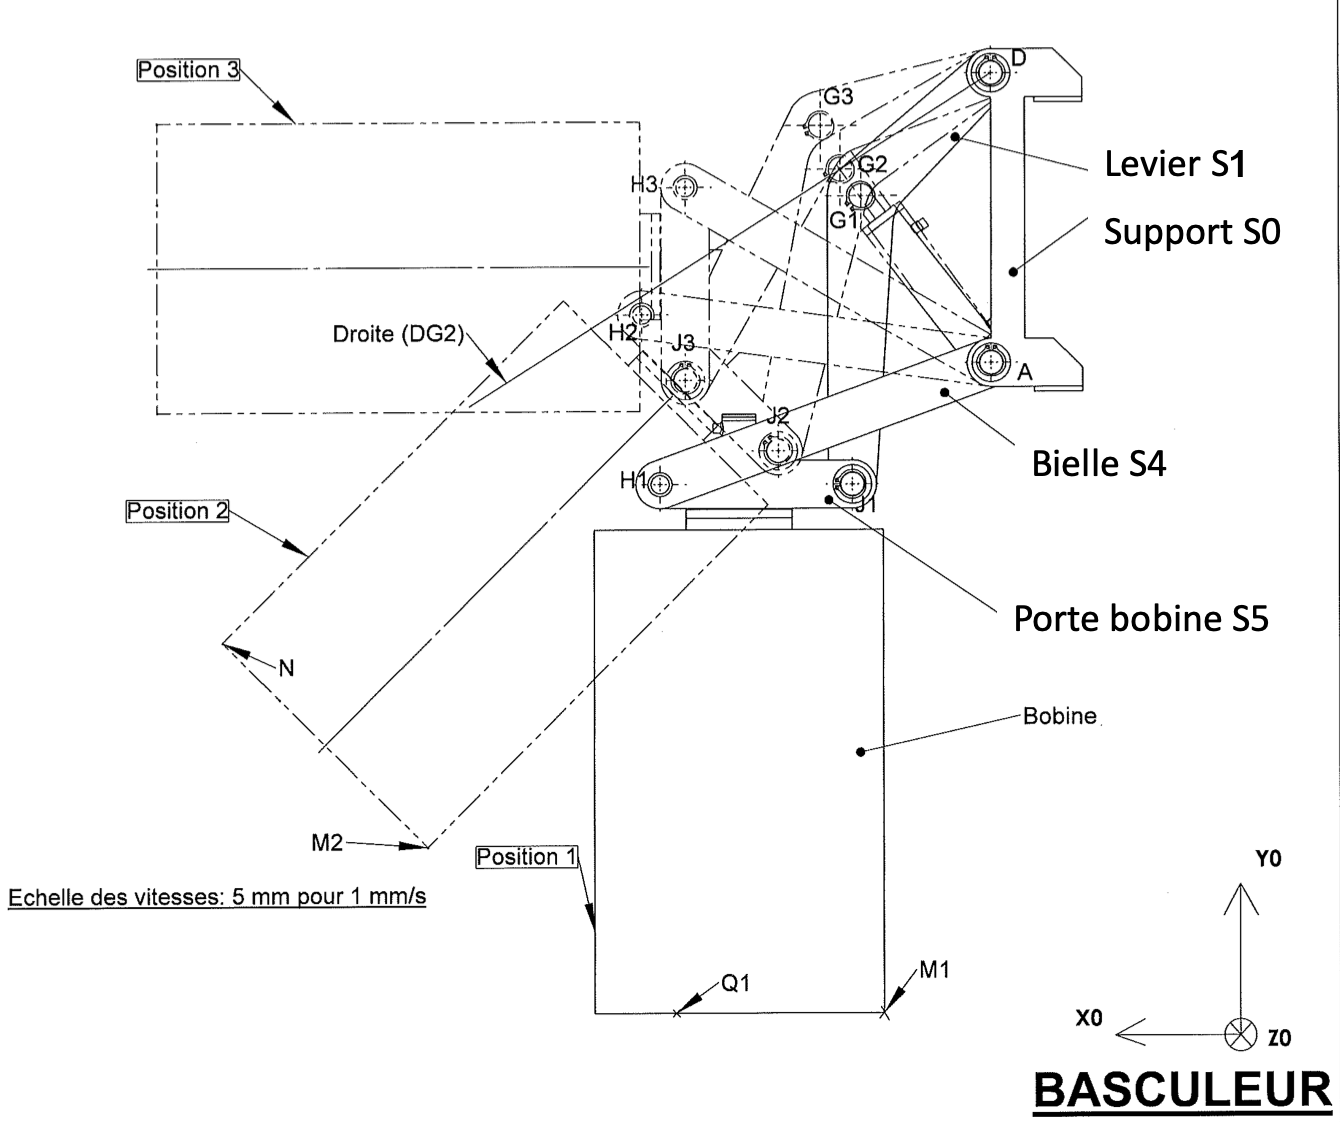
\includegraphics[width=0.9\linewidth]{img/DR06}
\end{center}}{\begin{center}
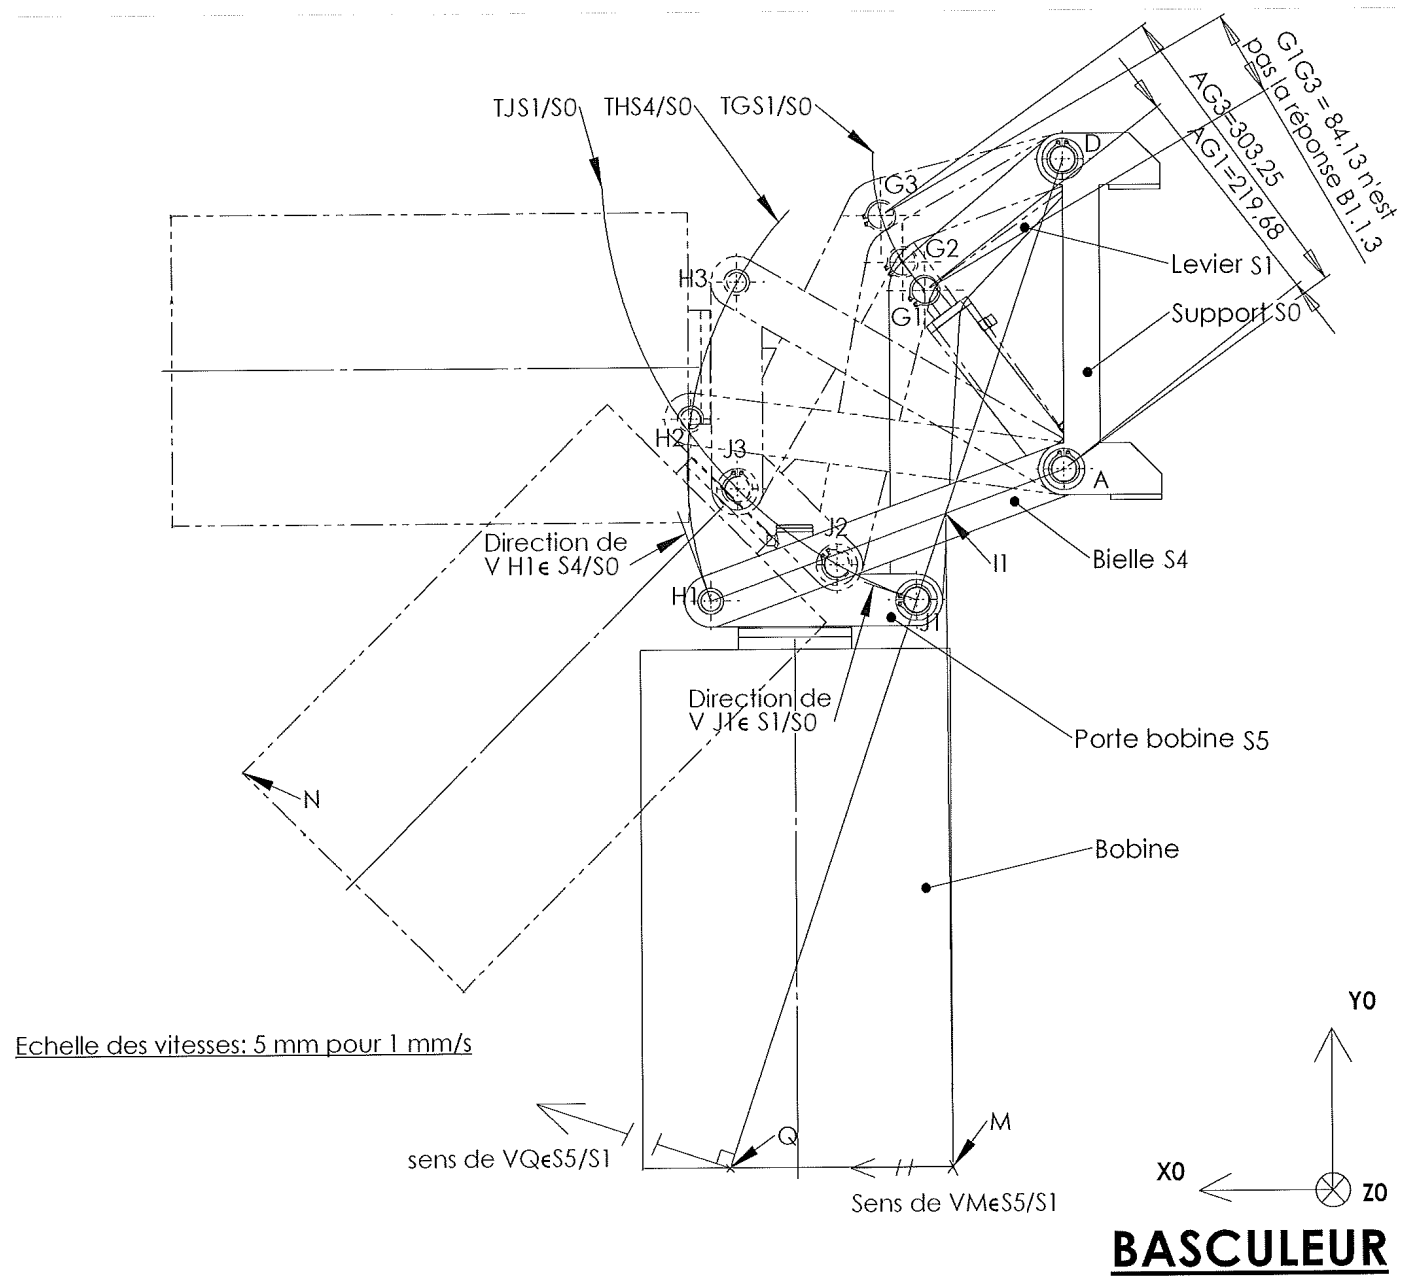
\includegraphics[width=0.9\linewidth]{img/DR06_cor}
\end{center}
$C_u=AG_3-AG_1=(61-44)\times 5=85mm$

Le vérin choisit ayant une course de $100mm$, il est compatible.
}

\reponse{3}{}{Le film plastique de la bobine risque la déchirure à cause du frottement. Si la bobine est plus grande, elle risque de talonner (descendre plus bas que le sol). L'utilisateur devra alors lever la bobine avant de la faire basculer horizontalement.}

\reponse[9]{8}{\begin{center}
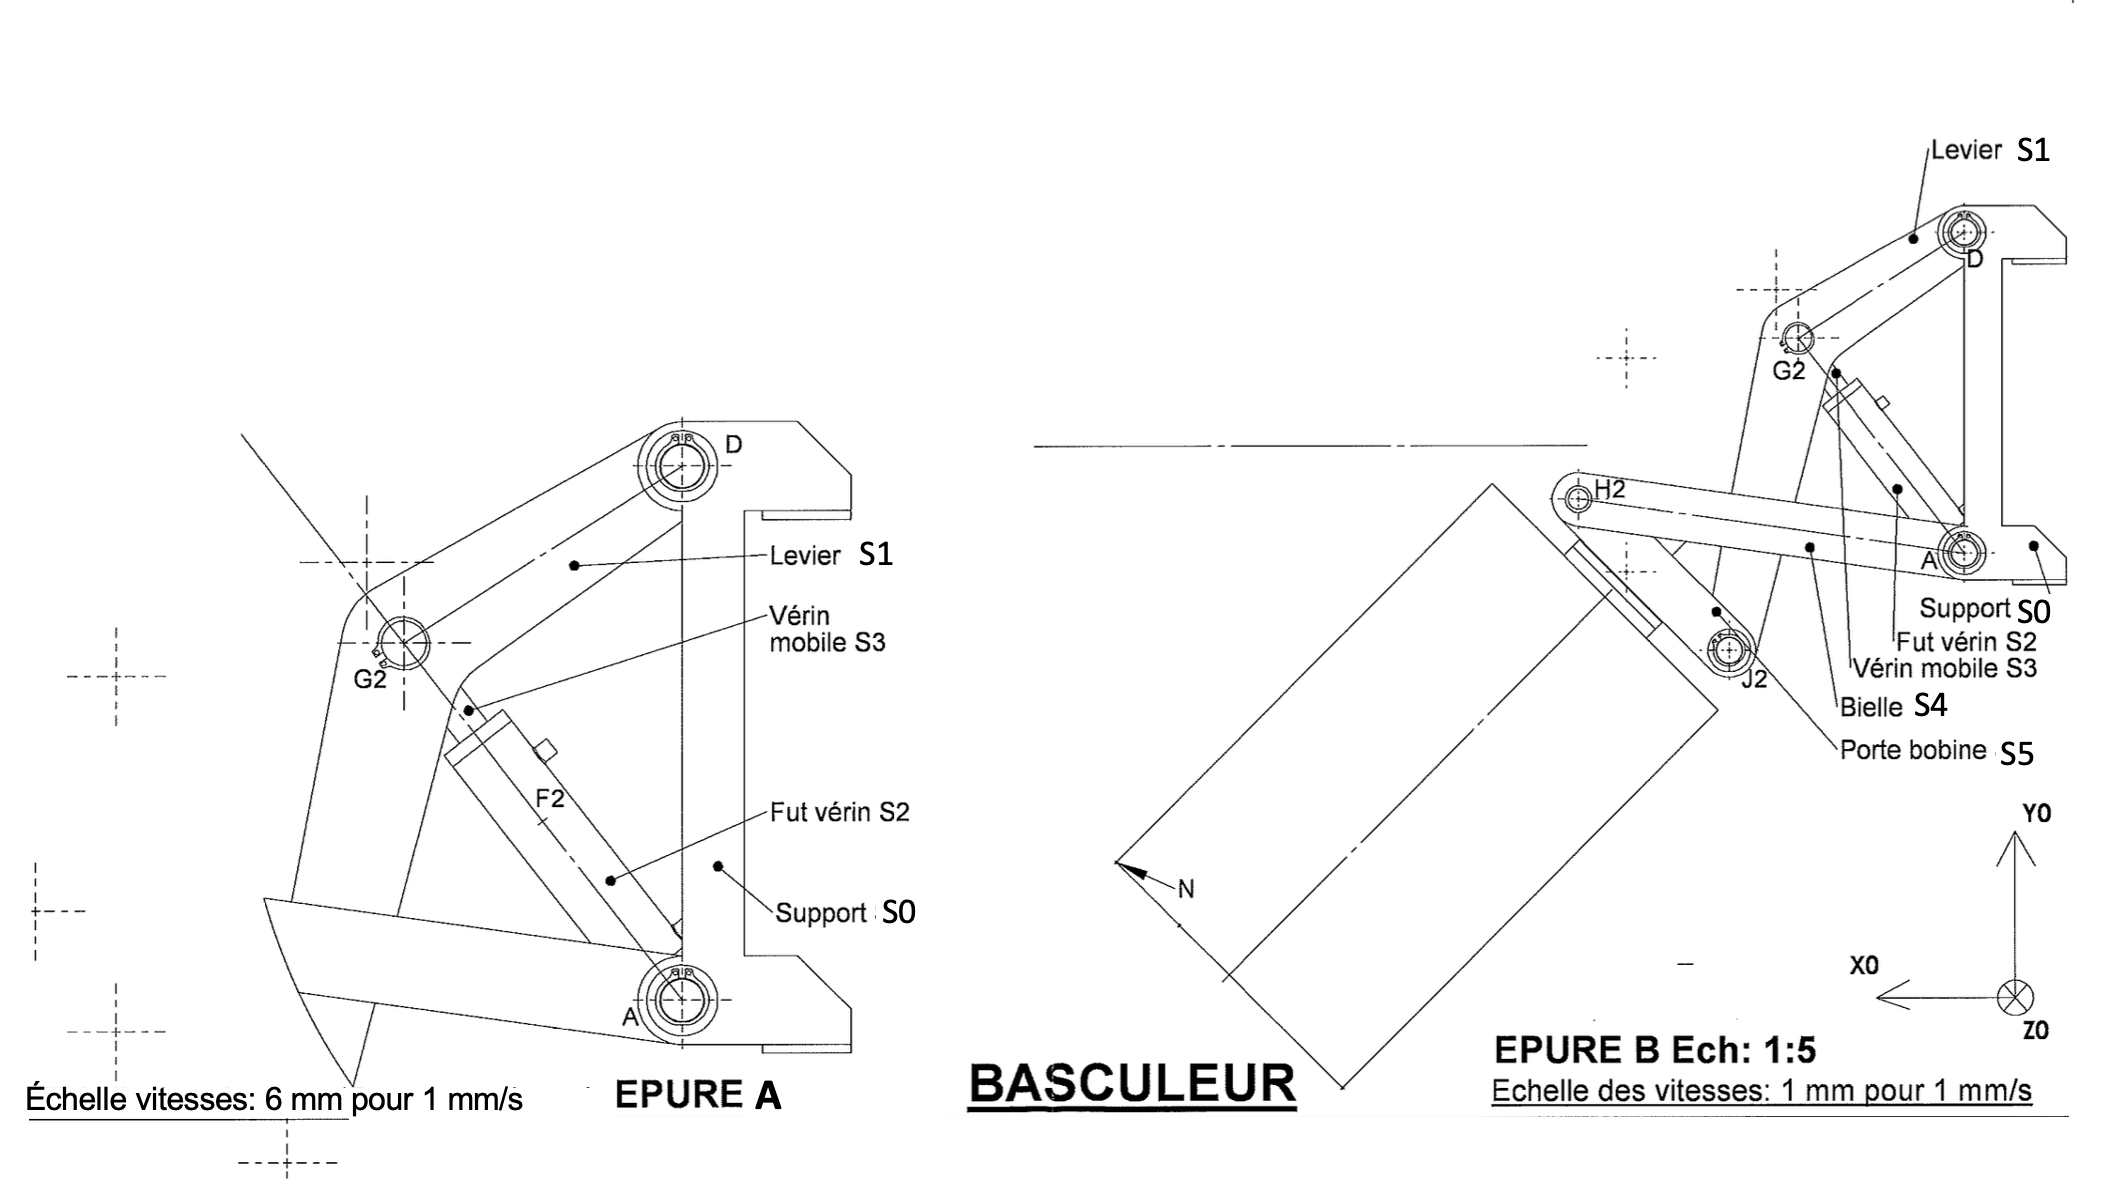
\includegraphics[width=1.3\linewidth,angle=90]{img/DR07}
\end{center}}{\begin{center}
  \def\svgwidth{0.9\linewidth}
  \input{img/DR07_cor.pdf_tex}
 \end{center}
}

\reponse{3}{}{
$\overrightarrow{V_{G_2\in S1/S0}}=\overrightarrow{V_{G_2\in S1/S3}}+\overrightarrow{V_{G_2\in S3/S2}}+\overrightarrow{V_{G_2\in S2/S0}}
$

$\overrightarrow{V_{G_2\in S1/S3}}=\overrightarrow{0}$

$\left\|\overrightarrow{V_{G_2\in S1/S0}}\right\|\approx11mm\cdot s^{-1}$

$\overrightarrow{V_{J_2\in S5/S1}}=\overrightarrow{0}$

Donc, $\overrightarrow{V_{J_2\in S5/S0}}=\overrightarrow{V_{J_2\in S1/S0}}$

$\overrightarrow{V_{H_2\in S5/S4}}=\overrightarrow{0}$

Donc, $\overrightarrow{V_{H_2\in S5/S0}}=\overrightarrow{V_{H_2\in S4/S0}}$

On trouve donc $\|\overrightarrow{V_{N\in S5/S0}}\|=130mm\cdot s^{-1}$
}

\reponse{3}{}{$\|\overrightarrow{V_{N\in S5/S0}}=130mm\cdot s^{-1}<200mm\cdot s^{-1}$, donc le cahier des charges est respecté.}

\reponse{10}{}{\begin{center}
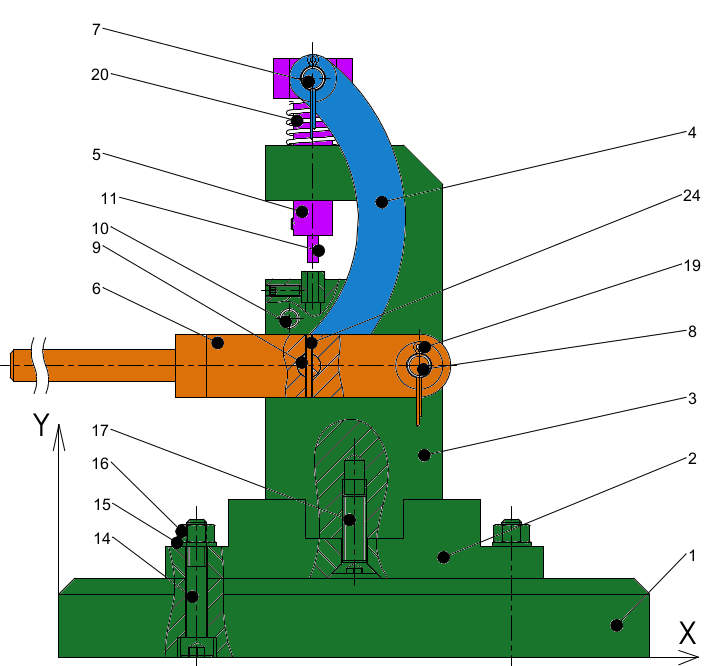
\includegraphics[width=0.9\linewidth]{img/10978-presse-ensemble_correction}
\end{center}}

\reponse{10}{}{\begin{center}
  \def\svgwidth{0.9\linewidth}
  \input{img/10978-presse-ensemble_liaisons.pdf_tex}
 \end{center}}

\reponse{10}{}{\begin{center}
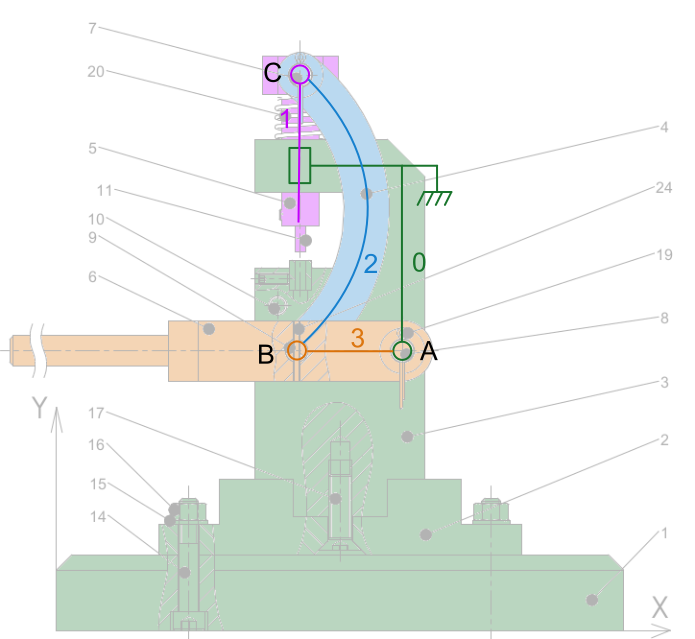
\includegraphics[width=0.7\linewidth]{img/10978-presse-ensemble_cinematique}
\end{center}}

\end{document}
